\chapter{Case study: geostatistics on neolithic settlements in Tavoliere}

    \begin{chaptersum}
        Sommario in italiano
    \end{chaptersum}

    The geostatistical system described in this chapter has been structured using the processed spatial data collected during almost ten years of surveying of the settlements in the Tavoliere plain. The existence of buried settlements ranging from neolithic period to middle ages has been proved by field and aerial surveys and by historical records. Given the variety and widespread distribution of the settlements across about \SI{150}{\hectare}, aerial and geophysical methods assured the best results, and heavily contributed to collect the data useful to an accurate landscape archaeology study \cite[pp.~45--48]{remote-ciminale}.

    \section{General features of the settlements}
        As extensively reported in literature \cite{intro-tavoliere}, the 256 sites form one of the densest concentrations of prehistoric settlements in Europe, lying within a plain approximately \SI{50}{\kilo\meter} by \SI{80}{\kilo\meter} at its broadest and longest points. The natural boundaries of this area are marked from rivers Fortore and Ofanto --- north and south --- and the Gulf of Manfredonia and Appennine foothills --- east and west.\\
        The settlements are large or small villages, normally surrounded by one or more ditches, with the interior generally filled with a number of internal compounds. The majority of the sites occupied level ground. Refer to published materials for further details.

        \subsection{Published data and the work of J. D. B. Jones}

            \subsubsection{Spatial analysis}

        \subsection{Modern spatial investigations}
            \begin{table}
    \centering
    \begin{tabular}{cccc}
        \toprule
        Layer type & Description          & Features & Scale \\
        \otoprule
        raster     & magnetic prospection & ---      & TODO  \\
        raster     & aerial photography   & ---      & TODO  \\
        vector     & ditches / compounds / areas & 1300   & ---   \\
        \bottomrule
    \end{tabular}
    \caption[List of layers in Tavoliere neolithic GIS project]{Details of the layers in the Tavoliere GIS project.
    \label{tab:layers}
    }
\end{table}
% tif con griglia magnetogramma
% magnetogramma tif
% foto ortorettificata
% layer vect punti GPS estremi magnetogramma

% viene prima inserito magnetogramma con griglia in unico file raster, poi derivato magnetogramma senza griglia
% georeferenziazione viene operata su magnetogramma con griglia

% WMS SIT Puglia
% WMS Geoportale Nazionale
% cartografia IGM 25000
% carta geologica

            After the post-processing, all the data have been placed in a GIS environment, currently containing XXX different raster layers and a single vector layer (\fref{tab:layers}). These vector layers refer to the latest study in chronological order, carried out by dott.ssa Angela Laterza in 2013,
            % TODO: add bib reference to Angelica's thesis
            who completely digitized the structures contained in 23 neolithic settlements. The whole digitalization process took as long as 320 hours and consisted in manually tracing the borders of the visible structures (\emph{ditches} and \emph{compounds}) and, as a separate geometry, the respective area for each of them; the operator has been employed for about two months, and has produced about 1300 geometries; \fref{fig:scheme-derive} shows the whole process.

            \begin{figure}[htp]
                \resizebox{1.1\textwidth}{!}{%
                    \input{tab/dot-geo-workflow}
                }
                \caption[Data deriving workflow for the Tavoliere project]{Data derivation workflow for the case study. Raster layers (\textsf{rs}) are the source of all derived vector data (\textsf{vt}). Bold lines represents a manual process, while dashed ones an automated process. Red lines define the area of intervention of the current work.}
                \label{fig:scheme-derive}
            \end{figure}

    \section{The GIS approach to statistics}
        The first step in statistical analysis at any level is to build a suitable set of data. In this case study, vector shapes of ditches and compounds can be considered as \emph{primary} data, while area geometries as \emph{derived} data.
        The statistical and spatial approach to the study of neolithic --- or, in general, prehistoric --- settlements data is well documented in literature \cite{arch-location-model}, and the strict relation between the morphology of the natural environment and the ancient societies enforces the use of GIS systems when deriving data.\\
        Moving from the standard geophysical survey workflow to a spatial analysis context during the study of the settlements has generated some necessities, which need to be added to the critical points already defined in \fref{sec:gis-data-management}:

        \begin{description}
            \item[automate derived data creation] the set of derived data may be generated automatically, since it consists of geometries describing the same characteristic on every shape (e.g.\ the internal area of a ditch, for all ditches);
            \item[automate calculations] most of the processes operated on data take a feature of the element (e.g. the perimeter), save it in a database field, retrieves all of them and make calculations; this is a repetitive task which could be done more efficiently;
            \item[platform independent results] the results must be reproducible by any researcher on any platform, and the dynamics of calculations must be public; the structure of the project should enable other researchers to contribute and improve the algorithms.
        \end{description}

        Given that, some objectives have been defined to improve the current workflow and speed up the process, trying to gain in the same time more precision, accuracy and reproducibility; the following subsections will explain how every objective has been achieved in detail.

        \subsection{Bulk distinguishing ditches and compounds}
            In the current approach, ditches and compounds geometries are distinguished by attributes (the \textsf{Ditch\_comp} field in the Shapefile is respectively set to $1$ or $2$), manually added by the operator to each structure in the Shapefile.

            \begin{wrapfigure}{l}{0.5\textwidth}
                \centering
                \vspace{-0.05\textheight}
                \begin{tikzpicture}[x=1mm,y=1mm,scale=0.005]
                    \input{tab/dot-flow-map}
                \end{tikzpicture}
                \caption[Flow chart: the logic of bulk distinguishing ditches and compounds]{If any of the ditches and compounds are sharing the same color (class), class total number $k$ must be changed. At the end, geometry type is saved as an attribute in the shapefile.}
                \label{fig:flow-map}
                \vspace{-0.03\textheight}
            \end{wrapfigure}

            This operation has been semi-automated using the Jenks Natural Breaks classification method \cite{jenks1977}. Virtually any classification could have been chosen (quantile, standard deviation), but Jenks Natural Breaks has gained popularity in the last 20 years as a tool for coloring map objects based on objects properties (\emph{choropleth maps}), and it is a well known and tested tool\footnote{Some criticism has recently raised around the use of Jenks Natural Breaks for the classification of \emph{all} kinds of data; alternative solutions have been found for some distributions --- as heavy-tailed ones \cite{jenks-tail} --- but this is not the case, and Jenks has been experimentally proved as the most appropriate choice.}. It aims to present a series of break values that best represent the actual breaks observed in the data as opposed to some arbitrary classificatory scheme (i.e. equal interval); in this way the actual clustering of data values is preserved.

            In the case study, geometries have been classified by perimeter values (calculated and saved automatically from ditches and compounds shapes). The different coloring of the geometries on the map based on the newly created classes (\fref{fig:jenks-color}) helps the user to distinguish ditches from compounds at a glance.

            The process is semi-automated since the user have to manually select the ditches and, if necessary, change the class numbers to have a good fit. The flowchart in \fref{fig:flow-map} reports the logic of the process. At the end, the geometry types are saved as text attribute (literally \textsf{ditch} or \textsf{compound}) in a table containing the results of the processing (one row for each geometry); \fref{tab:jnb-results} shows sample data from the \emph{Anglisano} settlement.

            \begin{table}
                \centering
                \begin{tabular}{ccccc}
    \toprule
    ID & shapefile\_id & perimeter & class\_n & type\\
    \otoprule
    1 & 1 & 122.792532 & 3 & compound\\
    2 & 1 & 89.612125 & 2 & compound\\
    4 & 1 & 156.587759 & 3 & compound\\
    16 & 1 & 1606.964845 & 6 & ditch\\
    \bottomrule
\end{tabular}

                \caption[Sample geometry classification results from Anglisano settlements using Jenk Natural Breaks method]{Sample results from the classification of Anglisano settlement's structures by perimeter using the Jenks Natural Breaks method. The kind of structure is saved as text attribute in the \textsf{type} column. The \textsf{shapefile\_id} column binds the geometries to the respective settlement.}
                \label{tab:jnb-results}
            \end{table}

            \begin{figure}
                \centering
                \rotatebox{180}{
                    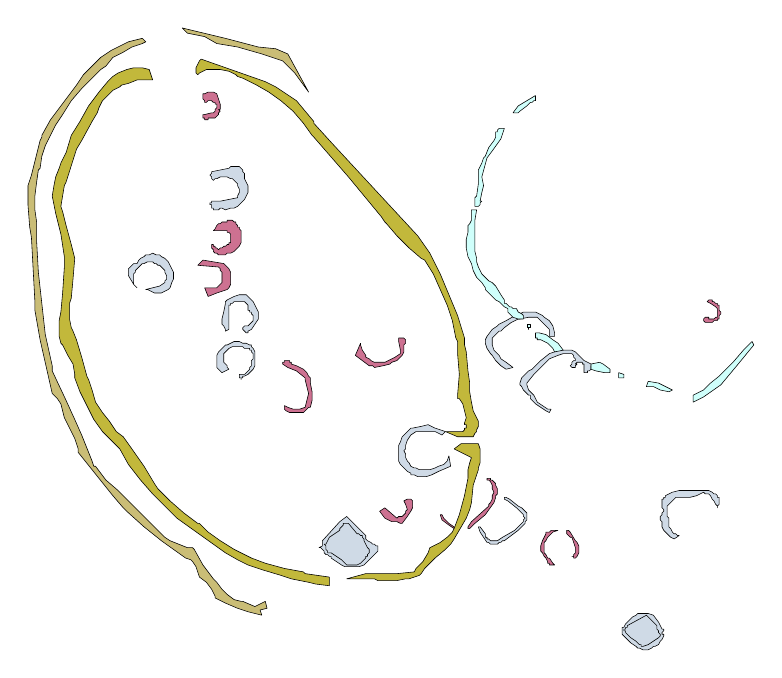
\begin{tikzpicture}[x=1mm,y=1mm,scale=0.22]
                        \definecolor{cff0000}{RGB}{207,240,0}
\definecolor{c2b83ba}{RGB}{194,184,59}
\definecolor{cabdda4}{RGB}{202,189,118}
\definecolor{cffffbf}{RGB}{207,255,251}
\definecolor{cfdae61}{RGB}{207,218,230}
\definecolor{cd7191c}{RGB}{205,113,145}

\begin{scope}[draw=black,fill=cd7191c,line join=round,line width=0.208pt]
  \path[draw,fill] (545.0000,190.0000) -- (544.0000,191.0000) --
    (543.0000,191.0000) -- (543.0000,190.0000) -- (543.0000,189.0000) --
    (544.0000,188.0000) -- (545.0000,187.0000) -- (546.0000,187.0000) --
    (548.0000,181.0000) -- (548.0000,180.0000) -- (548.0000,179.0000) --
    (548.0000,178.0000) -- (547.0000,177.0000) -- (547.0000,176.0000) --
    (546.0000,176.0000) -- (547.0000,176.0000) -- (547.0000,175.0000) --
    (548.0000,175.0000) -- (549.0000,176.0000) -- (550.0000,178.0000) --
    (550.0000,180.0000) -- (550.0000,182.0000) -- (549.0000,184.0000) --
    (548.0000,185.0000) -- (545.0000,190.0000);
  \path[draw,fill] (538.0000,191.0000) -- (537.0000,191.0000) --
    (536.0000,191.0000) -- (535.0000,191.0000) -- (534.0000,191.0000) --
    (533.0000,190.0000) -- (531.0000,190.0000) -- (531.0000,189.0000) --
    (529.0000,185.0000) -- (528.0000,182.0000) -- (528.0000,181.0000) --
    (528.0000,179.0000) -- (529.0000,178.0000) -- (530.0000,176.0000) --
    (531.0000,175.0000) -- (532.0000,173.0000) -- (532.0000,172.0000) --
    (533.0000,172.0000) -- (533.0000,171.0000) -- (534.0000,171.0000) --
    (535.0000,171.0000) -- (536.0000,171.0000) -- (535.0000,172.0000) --
    (533.0000,175.0000) -- (532.0000,175.0000) -- (531.0000,177.0000) --
    (530.0000,178.0000) -- (530.0000,180.0000) -- (530.0000,182.0000) --
    (530.0000,183.0000) -- (530.0000,184.0000) -- (531.0000,185.0000) --
    (532.0000,187.0000) -- (533.0000,188.0000) -- (534.0000,189.0000) --
    (535.0000,190.0000) -- (538.0000,191.0000);
  \path[draw,fill] (339.0000,356.0000) -- (338.0000,356.0000) --
    (338.0000,355.0000) -- (338.0000,354.0000) -- (339.0000,353.0000) --
    (339.0000,352.0000) -- (340.0000,351.0000) -- (341.0000,351.0000) --
    (342.0000,350.0000) -- (343.0000,350.0000) -- (344.0000,350.0000) --
    (345.0000,350.0000) -- (346.0000,350.0000) -- (347.0000,351.0000) --
    (349.0000,351.0000) -- (351.0000,352.0000) -- (352.0000,353.0000) --
    (353.0000,354.0000) -- (354.0000,355.0000) -- (355.0000,357.0000) --
    (355.0000,359.0000) -- (355.0000,360.0000) -- (355.0000,362.0000) --
    (355.0000,364.0000) -- (354.0000,365.0000) -- (354.0000,366.0000) --
    (353.0000,366.0000) -- (353.0000,367.0000) -- (352.0000,368.0000) --
    (352.0000,369.0000) -- (351.0000,369.0000) -- (350.0000,370.0000) --
    (349.0000,370.0000) -- (348.0000,370.0000) -- (347.0000,370.0000) --
    (347.0000,369.0000) -- (346.0000,369.0000) -- (345.0000,369.0000) --
    (344.0000,369.0000) -- (343.0000,368.0000) -- (342.0000,368.0000) --
    (341.0000,367.0000) -- (340.0000,365.0000) -- (339.0000,364.0000) --
    (343.0000,364.0000) -- (347.0000,364.0000) -- (347.0000,363.0000) --
    (348.0000,363.0000) -- (349.0000,362.0000) -- (349.0000,361.0000) --
    (349.0000,360.0000) -- (349.0000,359.0000) -- (349.0000,358.0000) --
    (349.0000,357.0000) -- (348.0000,357.0000) -- (348.0000,356.0000) --
    (347.0000,356.0000) -- (346.0000,355.0000) -- (345.0000,355.0000) --
    (344.0000,354.0000) -- (343.0000,354.0000) -- (342.0000,353.0000) --
    (341.0000,354.0000) -- (340.0000,354.0000) -- (340.0000,355.0000) --
    (339.0000,355.0000) -- (339.0000,356.0000);
  \path[draw,fill] (330.0000,344.0000) -- (342.0000,343.0000) --
    (343.0000,342.0000) -- (343.0000,341.0000) -- (344.0000,340.0000) --
    (344.0000,339.0000) -- (344.0000,337.0000) -- (344.0000,336.0000) --
    (344.0000,335.0000) -- (344.0000,334.0000) -- (343.0000,333.0000) --
    (342.0000,332.0000) -- (341.0000,331.0000) -- (340.0000,331.0000) --
    (334.0000,331.0000) -- (336.0000,326.0000) -- (341.0000,328.0000) --
    (347.0000,330.0000) -- (348.0000,331.0000) -- (349.0000,333.0000) --
    (349.0000,335.0000) -- (349.0000,336.0000) -- (349.0000,338.0000) --
    (349.0000,340.0000) -- (348.0000,342.0000) -- (347.0000,343.0000) --
    (345.0000,345.0000) -- (333.0000,347.0000) -- (330.0000,344.0000);
  \path[draw,fill] (424.0000,299.0000) -- (421.0000,292.0000) --
    (425.0000,289.0000) -- (429.0000,286.0000) -- (431.0000,286.0000) --
    (432.0000,285.0000) -- (437.0000,286.0000) -- (441.0000,287.0000) --
    (442.0000,288.0000) -- (445.0000,289.0000) -- (446.0000,290.0000) --
    (447.0000,291.0000) -- (448.0000,292.0000) -- (449.0000,294.0000) --
    (449.0000,295.0000) -- (449.0000,297.0000) -- (449.0000,298.0000) --
    (450.0000,299.0000) -- (450.0000,300.0000) -- (450.0000,301.0000) --
    (449.0000,302.0000) -- (448.0000,302.0000) -- (447.0000,302.0000) --
    (446.0000,302.0000) -- (446.0000,301.0000) -- (446.0000,300.0000) --
    (447.0000,295.0000) -- (447.0000,293.0000) -- (444.0000,291.0000) --
    (438.0000,288.0000) -- (436.0000,288.0000) -- (434.0000,288.0000) --
    (432.0000,288.0000) -- (430.0000,289.0000) -- (429.0000,290.0000) --
    (427.0000,291.0000) -- (427.0000,292.0000) -- (425.0000,295.0000) --
    (424.0000,298.0000) -- (424.0000,299.0000);
  \path[draw,fill] (380.0000,263.0000) -- (380.0000,261.0000) --
    (381.0000,260.0000) -- (383.0000,259.0000) -- (385.0000,259.0000) --
    (387.0000,259.0000) -- (389.0000,259.0000) -- (391.0000,259.0000) --
    (392.0000,260.0000) -- (393.0000,261.0000) -- (394.0000,262.0000) --
    (395.0000,262.0000) -- (396.0000,266.0000) -- (396.0000,271.0000) --
    (395.0000,276.0000) -- (395.0000,279.0000) -- (394.0000,280.0000) --
    (393.0000,282.0000) -- (391.0000,284.0000) -- (389.0000,285.0000) --
    (387.0000,286.0000) -- (384.0000,287.0000) -- (384.0000,288.0000) --
    (383.0000,288.0000) -- (383.0000,289.0000) -- (382.0000,289.0000) --
    (381.0000,289.0000) -- (380.0000,289.0000) -- (380.0000,288.0000) --
    (379.0000,288.0000) -- (379.0000,287.0000) -- (382.0000,285.0000) --
    (387.0000,283.0000) -- (392.0000,279.0000) -- (392.0000,278.0000) --
    (393.0000,274.0000) -- (394.0000,270.0000) -- (393.0000,266.0000) --
    (392.0000,262.0000) -- (389.0000,261.0000) -- (385.0000,261.0000) --
    (382.0000,262.0000) -- (380.0000,263.0000);
  \path[draw,fill] (334.0000,431.0000) -- (333.0000,431.0000) --
    (333.0000,430.0000) -- (333.0000,429.0000) -- (334.0000,429.0000) --
    (334.0000,428.0000) -- (335.0000,428.0000) -- (336.0000,428.0000) --
    (336.0000,429.0000) -- (337.0000,429.0000) -- (338.0000,429.0000) --
    (339.0000,429.0000) -- (340.0000,429.0000) -- (341.0000,430.0000) --
    (342.0000,431.0000) -- (342.0000,432.0000) -- (343.0000,433.0000) --
    (342.0000,434.0000) -- (343.0000,434.0000) -- (343.0000,437.0000) --
    (342.0000,440.0000) -- (341.0000,443.0000) -- (339.0000,444.0000) --
    (337.0000,444.0000) -- (336.0000,444.0000) -- (334.0000,443.0000) --
    (333.0000,443.0000) -- (333.0000,442.0000) -- (333.0000,441.0000) --
    (333.0000,440.0000) -- (334.0000,439.0000) -- (334.0000,438.0000) --
    (335.0000,438.0000) -- (336.0000,439.0000) -- (337.0000,439.0000) --
    (338.0000,439.0000) -- (339.0000,438.0000) -- (340.0000,438.0000) --
    (340.0000,437.0000) -- (341.0000,437.0000) -- (341.0000,436.0000) --
    (341.0000,435.0000) -- (340.0000,434.0000) -- (340.0000,433.0000) --
    (339.0000,432.0000) -- (338.0000,432.0000) -- (334.0000,431.0000);
  \path[draw,fill] (438.0000,204.0000) -- (435.0000,202.0000) --
    (438.0000,198.0000) -- (442.0000,196.0000) -- (445.0000,196.0000) --
    (447.0000,195.0000) -- (448.0000,195.0000) -- (451.0000,199.0000) --
    (453.0000,202.0000) -- (454.0000,204.0000) -- (454.0000,205.0000) --
    (454.0000,206.0000) -- (454.0000,207.0000) -- (454.0000,208.0000) --
    (453.0000,209.0000) -- (451.0000,209.0000) -- (449.0000,208.0000) --
    (450.0000,206.0000) -- (451.0000,203.0000) -- (450.0000,202.0000) --
    (450.0000,201.0000) -- (449.0000,200.0000) -- (448.0000,199.0000) --
    (446.0000,199.0000) -- (445.0000,198.0000) -- (438.0000,204.0000);
  \path[draw,fill] (486.0000,193.0000) -- (486.0000,192.0000) --
    (487.0000,192.0000) -- (490.0000,195.0000) -- (496.0000,200.0000) --
    (501.0000,207.0000) -- (502.0000,210.0000) -- (502.0000,211.0000) --
    (503.0000,212.0000) -- (503.0000,214.0000) -- (503.0000,215.0000) --
    (502.0000,217.0000) -- (502.0000,218.0000) -- (501.0000,219.0000) --
    (500.0000,220.0000) -- (499.0000,220.0000) -- (499.0000,221.0000) --
    (498.0000,221.0000) -- (497.0000,221.0000) -- (497.0000,220.0000) --
    (498.0000,220.0000) -- (499.0000,219.0000) -- (500.0000,217.0000) --
    (500.0000,215.0000) -- (501.0000,213.0000) -- (500.0000,211.0000) --
    (500.0000,209.0000) -- (499.0000,207.0000) -- (498.0000,206.0000) --
    (498.0000,205.0000) -- (488.0000,196.0000) -- (486.0000,193.0000);
  \path[draw,fill] (470.0000,200.0000) -- (471.0000,197.0000) --
    (475.0000,194.0000) -- (478.0000,192.0000) -- (478.0000,193.0000) --
    (475.0000,195.0000) -- (472.0000,198.0000) -- (471.0000,200.0000) --
    (470.0000,200.0000);
  \path[draw,fill] (624.0000,323.0000) -- (626.0000,322.0000) --
    (629.0000,320.0000) -- (630.0000,319.0000) -- (630.0000,318.0000) --
    (630.0000,317.0000) -- (630.0000,316.0000) -- (630.0000,315.0000) --
    (630.0000,314.0000) -- (629.0000,314.0000) -- (628.0000,313.0000) --
    (627.0000,313.0000) -- (626.0000,313.0000) -- (625.0000,313.0000) --
    (625.0000,314.0000) -- (624.0000,314.0000) -- (623.0000,314.0000) --
    (622.0000,313.0000) -- (622.0000,312.0000) -- (623.0000,311.0000) --
    (624.0000,311.0000) -- (626.0000,311.0000) -- (627.0000,311.0000) --
    (628.0000,312.0000) -- (630.0000,312.0000) -- (630.0000,313.0000) --
    (631.0000,313.0000) -- (631.0000,314.0000) -- (631.0000,315.0000) --
    (632.0000,316.0000) -- (632.0000,317.0000) -- (631.0000,318.0000) --
    (631.0000,319.0000) -- (631.0000,320.0000) -- (631.0000,321.0000) --
    (630.0000,321.0000) -- (630.0000,322.0000) -- (629.0000,322.0000) --
    (628.0000,323.0000) -- (627.0000,323.0000) -- (627.0000,324.0000) --
    (626.0000,324.0000) -- (625.0000,324.0000) -- (624.0000,323.0000);
\end{scope}
\begin{scope}[draw=black,fill=cfdae61,line join=round,line width=0.208pt]
  \path[draw,fill] (579.0000,127.0000) -- (580.0000,126.0000) --
    (583.0000,124.0000) -- (584.0000,123.0000) -- (585.0000,123.0000) --
    (587.0000,122.0000) -- (588.0000,122.0000) -- (590.0000,122.0000) --
    (592.0000,123.0000) -- (593.0000,124.0000) -- (594.0000,124.0000) --
    (596.0000,125.0000) -- (597.0000,127.0000) -- (598.0000,128.0000) --
    (599.0000,130.0000) -- (599.0000,131.0000) -- (598.0000,131.0000) --
    (598.0000,132.0000) -- (599.0000,133.0000) -- (599.0000,134.0000) --
    (598.0000,134.0000) -- (596.0000,138.0000) -- (593.0000,142.0000) --
    (590.0000,143.0000) -- (588.0000,143.0000) -- (587.0000,143.0000) --
    (586.0000,143.0000) -- (584.0000,143.0000) -- (583.0000,142.0000) --
    (581.0000,141.0000) -- (580.0000,140.0000) -- (579.0000,139.0000) --
    (577.0000,137.0000) -- (576.0000,135.0000) -- (575.0000,135.0000) --
    (575.0000,134.0000) -- (575.0000,133.0000) -- (575.0000,132.0000) --
    (575.0000,131.0000) -- (579.0000,127.0000);
  \path[draw,fill] (578.0000,136.0000) -- (589.0000,142.0000) --
    (593.0000,138.0000) -- (594.0000,137.0000) -- (595.0000,136.0000) --
    (595.0000,135.0000) -- (595.0000,134.0000) -- (596.0000,133.0000) --
    (596.0000,132.0000) -- (597.0000,131.0000) -- (597.0000,130.0000) --
    (596.0000,129.0000) -- (593.0000,127.0000) -- (590.0000,125.0000) --
    (587.0000,124.0000) -- (586.0000,124.0000) -- (586.0000,125.0000) --
    (585.0000,125.0000) -- (583.0000,127.0000) -- (580.0000,129.0000) --
    (578.0000,131.0000) -- (577.0000,132.0000) -- (577.0000,133.0000) --
    (576.0000,133.0000) -- (576.0000,134.0000) -- (577.0000,134.0000) --
    (577.0000,135.0000) -- (578.0000,135.0000) -- (578.0000,136.0000);
  \path[draw,fill] (608.0000,188.0000) -- (607.0000,188.0000) --
    (606.0000,189.0000) -- (605.0000,189.0000) -- (604.0000,190.0000) --
    (603.0000,192.0000) -- (602.0000,193.0000) -- (602.0000,194.0000) --
    (602.0000,196.0000) -- (602.0000,197.0000) -- (602.0000,198.0000) --
    (601.0000,199.0000) -- (601.0000,201.0000) -- (601.0000,202.0000) --
    (601.0000,203.0000) -- (601.0000,205.0000) -- (602.0000,206.0000) --
    (603.0000,207.0000) -- (604.0000,208.0000) -- (605.0000,209.0000) --
    (606.0000,210.0000) -- (607.0000,210.0000) -- (608.0000,210.0000) --
    (609.0000,210.0000) -- (614.0000,210.0000) -- (618.0000,211.0000) --
    (622.0000,213.0000) -- (623.0000,212.0000) -- (625.0000,212.0000) --
    (626.0000,211.0000) -- (627.0000,209.0000) -- (628.0000,208.0000) --
    (629.0000,206.0000) -- (630.0000,205.0000) -- (630.0000,204.0000) --
    (630.0000,205.0000) -- (631.0000,206.0000) -- (631.0000,207.0000) --
    (631.0000,208.0000) -- (631.0000,209.0000) -- (631.0000,210.0000) --
    (630.0000,210.0000) -- (630.0000,211.0000) -- (629.0000,212.0000) --
    (628.0000,212.0000) -- (627.0000,213.0000) -- (625.0000,214.0000) --
    (620.0000,214.0000) -- (614.0000,214.0000) -- (613.0000,214.0000) --
    (612.0000,214.0000) -- (608.0000,214.0000) -- (604.0000,213.0000) --
    (600.0000,211.0000) -- (600.0000,210.0000) -- (599.0000,210.0000) --
    (599.0000,209.0000) -- (598.0000,209.0000) -- (598.0000,208.0000) --
    (598.0000,207.0000) -- (598.0000,206.0000) -- (598.0000,205.0000) --
    (598.0000,204.0000) -- (599.0000,203.0000) -- (599.0000,202.0000) --
    (598.0000,201.0000) -- (598.0000,200.0000) -- (597.0000,199.0000) --
    (597.0000,198.0000) -- (597.0000,197.0000) -- (598.0000,196.0000) --
    (598.0000,195.0000) -- (598.0000,193.0000) -- (599.0000,191.0000) --
    (600.0000,190.0000) -- (602.0000,188.0000) -- (603.0000,187.0000) --
    (605.0000,186.0000) -- (608.0000,188.0000);
  \path[draw,fill] (534.0000,261.0000) -- (532.0000,261.0000) --
    (529.0000,263.0000) -- (526.0000,265.0000) -- (524.0000,269.0000) --
    (523.0000,270.0000) -- (521.0000,272.0000) -- (520.0000,275.0000) --
    (520.0000,276.0000) -- (524.0000,281.0000) -- (529.0000,286.0000) --
    (533.0000,290.0000) -- (538.0000,292.0000) -- (541.0000,293.0000) --
    (542.0000,293.0000) -- (544.0000,293.0000) -- (545.0000,293.0000) --
    (546.0000,293.0000) -- (547.0000,292.0000) -- (547.0000,291.0000) --
    (548.0000,290.0000) -- (548.0000,289.0000) -- (547.0000,289.0000) --
    (546.0000,288.0000) -- (546.0000,287.0000) -- (545.0000,286.0000) --
    (546.0000,285.0000) -- (547.0000,285.0000) -- (548.0000,285.0000) --
    (548.0000,286.0000) -- (549.0000,287.0000) -- (548.0000,287.0000) --
    (549.0000,288.0000) -- (550.0000,288.0000) -- (551.0000,288.0000) --
    (552.0000,288.0000) -- (552.0000,287.0000) -- (553.0000,287.0000) --
    (553.0000,283.0000) -- (553.0000,282.0000) -- (554.0000,282.0000) --
    (555.0000,282.0000) -- (555.0000,283.0000) -- (556.0000,283.0000) --
    (557.0000,284.0000) -- (557.0000,285.0000) -- (557.0000,286.0000) --
    (558.0000,286.0000) -- (557.0000,287.0000) -- (553.0000,289.0000) --
    (550.0000,292.0000) -- (548.0000,294.0000) -- (546.0000,295.0000) --
    (542.0000,295.0000) -- (538.0000,295.0000) -- (536.0000,294.0000) --
    (533.0000,293.0000) -- (528.0000,289.0000) -- (523.0000,284.0000) --
    (521.0000,283.0000) -- (519.0000,281.0000) -- (517.0000,279.0000) --
    (516.0000,276.0000) -- (516.0000,275.0000) -- (517.0000,274.0000) --
    (518.0000,272.0000) -- (519.0000,271.0000) -- (520.0000,270.0000) --
    (521.0000,269.0000) -- (522.0000,269.0000) -- (522.0000,267.0000) --
    (525.0000,264.0000) -- (528.0000,262.0000) -- (531.0000,260.0000) --
    (533.0000,259.0000) -- (534.0000,261.0000);
  \path[draw,fill] (512.0000,285.0000) -- (508.0000,288.0000) --
    (505.0000,290.0000) -- (504.0000,292.0000) -- (501.0000,295.0000) --
    (500.0000,298.0000) -- (500.0000,299.0000) -- (500.0000,300.0000) --
    (500.0000,302.0000) -- (501.0000,303.0000) -- (502.0000,304.0000) --
    (503.0000,305.0000) -- (504.0000,306.0000) -- (505.0000,306.0000) --
    (507.0000,308.0000) -- (511.0000,311.0000) -- (515.0000,313.0000) --
    (516.0000,313.0000) -- (521.0000,314.0000) -- (526.0000,314.0000) --
    (527.0000,313.0000) -- (532.0000,308.0000) -- (533.0000,307.0000) --
    (533.0000,305.0000) -- (533.0000,304.0000) -- (533.0000,303.0000) --
    (534.0000,303.0000) -- (536.0000,303.0000) -- (536.0000,305.0000) --
    (535.0000,309.0000) -- (533.0000,312.0000) -- (530.0000,314.0000) --
    (529.0000,315.0000) -- (527.0000,316.0000) -- (525.0000,317.0000) --
    (523.0000,317.0000) -- (522.0000,317.0000) -- (520.0000,317.0000) --
    (518.0000,317.0000) -- (516.0000,316.0000) -- (515.0000,316.0000) --
    (508.0000,312.0000) -- (504.0000,310.0000) -- (503.0000,309.0000) --
    (500.0000,307.0000) -- (497.0000,303.0000) -- (496.0000,301.0000) --
    (496.0000,299.0000) -- (497.0000,296.0000) -- (499.0000,293.0000) --
    (500.0000,292.0000) -- (502.0000,289.0000) -- (505.0000,286.0000) --
    (508.0000,284.0000) -- (512.0000,285.0000);
  \path[draw,fill] (338.0000,398.0000) -- (338.0000,397.0000) --
    (337.0000,396.0000) -- (338.0000,395.0000) -- (338.0000,394.0000) --
    (339.0000,393.0000) -- (340.0000,394.0000) -- (341.0000,394.0000) --
    (343.0000,395.0000) -- (345.0000,395.0000) -- (347.0000,395.0000) --
    (349.0000,394.0000) -- (350.0000,394.0000) -- (351.0000,393.0000) --
    (352.0000,392.0000) -- (353.0000,391.0000) -- (353.0000,390.0000) --
    (354.0000,388.0000) -- (354.0000,387.0000) -- (354.0000,386.0000) --
    (353.0000,384.0000) -- (353.0000,383.0000) -- (348.0000,382.0000) --
    (343.0000,381.0000) -- (342.0000,381.0000) -- (338.0000,381.0000) --
    (338.0000,380.0000) -- (337.0000,380.0000) -- (337.0000,379.0000) --
    (338.0000,379.0000) -- (338.0000,378.0000) -- (338.0000,377.0000) --
    (339.0000,377.0000) -- (339.0000,376.0000) -- (340.0000,376.0000) --
    (341.0000,376.0000) -- (342.0000,376.0000) -- (343.0000,377.0000) --
    (344.0000,377.0000) -- (346.0000,376.0000) -- (349.0000,377.0000) --
    (351.0000,377.0000) -- (353.0000,378.0000) -- (355.0000,380.0000) --
    (356.0000,381.0000) -- (357.0000,382.0000) -- (358.0000,384.0000) --
    (359.0000,386.0000) -- (359.0000,388.0000) -- (359.0000,390.0000) --
    (358.0000,392.0000) -- (357.0000,394.0000) -- (357.0000,395.0000) --
    (357.0000,396.0000) -- (357.0000,397.0000) -- (356.0000,398.0000) --
    (356.0000,399.0000) -- (355.0000,400.0000) -- (354.0000,401.0000) --
    (353.0000,401.0000) -- (352.0000,401.0000) -- (351.0000,401.0000) --
    (350.0000,401.0000) -- (349.0000,401.0000) -- (348.0000,400.0000) --
    (338.0000,398.0000);
  \path[draw,fill] (348.0000,284.0000) -- (347.0000,285.0000) --
    (347.0000,286.0000) -- (346.0000,287.0000) -- (345.0000,288.0000) --
    (345.0000,289.0000) -- (345.0000,290.0000) -- (345.0000,292.0000) --
    (345.0000,293.0000) -- (346.0000,294.0000) -- (347.0000,295.0000) --
    (348.0000,296.0000) -- (350.0000,297.0000) -- (351.0000,297.0000) --
    (353.0000,297.0000) -- (354.0000,297.0000) -- (356.0000,297.0000) --
    (357.0000,296.0000) -- (358.0000,296.0000) -- (359.0000,296.0000) --
    (360.0000,296.0000) -- (360.0000,295.0000) -- (361.0000,295.0000) --
    (361.0000,294.0000) -- (362.0000,293.0000) -- (362.0000,292.0000) --
    (362.0000,291.0000) -- (362.0000,290.0000) -- (361.0000,289.0000) --
    (361.0000,288.0000) -- (361.0000,287.0000) -- (361.0000,286.0000) --
    (360.0000,285.0000) -- (360.0000,284.0000) -- (359.0000,283.0000) --
    (358.0000,282.0000) -- (357.0000,281.0000) -- (355.0000,281.0000) --
    (354.0000,281.0000) -- (354.0000,280.0000) -- (354.0000,279.0000) --
    (355.0000,279.0000) -- (355.0000,278.0000) -- (355.0000,279.0000) --
    (356.0000,279.0000) -- (356.0000,280.0000) -- (357.0000,280.0000) --
    (359.0000,281.0000) -- (360.0000,282.0000) -- (361.0000,283.0000) --
    (362.0000,284.0000) -- (363.0000,286.0000) -- (363.0000,288.0000) --
    (363.0000,289.0000) -- (363.0000,291.0000) -- (363.0000,292.0000) --
    (363.0000,293.0000) -- (363.0000,294.0000) -- (362.0000,296.0000) --
    (361.0000,297.0000) -- (361.0000,298.0000) -- (360.0000,298.0000) --
    (358.0000,299.0000) -- (357.0000,299.0000) -- (356.0000,299.0000) --
    (354.0000,300.0000) -- (352.0000,300.0000) -- (351.0000,300.0000) --
    (349.0000,299.0000) -- (347.0000,298.0000) -- (346.0000,298.0000) --
    (345.0000,297.0000) -- (343.0000,295.0000) -- (342.0000,294.0000) --
    (341.0000,292.0000) -- (341.0000,290.0000) -- (341.0000,288.0000) --
    (341.0000,287.0000) -- (341.0000,285.0000) -- (342.0000,284.0000) --
    (343.0000,283.0000) -- (344.0000,282.0000) -- (348.0000,284.0000);
  \path[draw,fill] (348.0000,307.0000) -- (348.0000,311.0000) --
    (348.0000,318.0000) -- (348.0000,319.0000) -- (348.0000,320.0000) --
    (348.0000,321.0000) -- (349.0000,321.0000) -- (349.0000,322.0000) --
    (350.0000,322.0000) -- (351.0000,323.0000) -- (352.0000,323.0000) --
    (353.0000,323.0000) -- (354.0000,323.0000) -- (355.0000,323.0000) --
    (356.0000,323.0000) -- (357.0000,323.0000) -- (358.0000,322.0000) --
    (359.0000,321.0000) -- (359.0000,320.0000) -- (359.0000,319.0000) --
    (359.0000,318.0000) -- (360.0000,318.0000) -- (360.0000,317.0000) --
    (361.0000,317.0000) -- (361.0000,316.0000) -- (362.0000,315.0000) --
    (362.0000,314.0000) -- (362.0000,313.0000) -- (362.0000,312.0000) --
    (361.0000,311.0000) -- (360.0000,310.0000) -- (359.0000,309.0000) --
    (357.0000,309.0000) -- (356.0000,308.0000) -- (356.0000,307.0000) --
    (357.0000,306.0000) -- (358.0000,305.0000) -- (359.0000,305.0000) --
    (359.0000,306.0000) -- (361.0000,307.0000) -- (363.0000,310.0000) --
    (365.0000,313.0000) -- (365.0000,314.0000) -- (365.0000,317.0000) --
    (363.0000,321.0000) -- (362.0000,323.0000) -- (361.0000,324.0000) --
    (359.0000,326.0000) -- (358.0000,327.0000) -- (356.0000,327.0000) --
    (354.0000,327.0000) -- (351.0000,326.0000) -- (349.0000,325.0000) --
    (347.0000,324.0000) -- (346.0000,323.0000) -- (346.0000,322.0000) --
    (345.0000,317.0000) -- (344.0000,313.0000) -- (344.0000,312.0000) --
    (344.0000,310.0000) -- (345.0000,309.0000) -- (346.0000,307.0000) --
    (346.0000,306.0000) -- (348.0000,307.0000);
  \path[draw,fill] (456.0000,248.0000) -- (462.0000,248.0000) --
    (467.0000,248.0000) -- (471.0000,246.0000) -- (473.0000,248.0000) --
    (467.0000,250.0000) -- (463.0000,252.0000) -- (459.0000,251.0000) --
    (454.0000,250.0000) -- (453.0000,250.0000) -- (451.0000,248.0000) --
    (448.0000,245.0000) -- (447.0000,242.0000) -- (446.0000,240.0000) --
    (446.0000,238.0000) -- (446.0000,236.0000) -- (446.0000,233.0000) --
    (446.0000,231.0000) -- (447.0000,229.0000) -- (449.0000,227.0000) --
    (451.0000,225.0000) -- (453.0000,224.0000) -- (453.0000,223.0000) --
    (455.0000,223.0000) -- (457.0000,222.0000) -- (460.0000,222.0000) --
    (462.0000,222.0000) -- (465.0000,223.0000) -- (467.0000,224.0000) --
    (469.0000,225.0000) -- (476.0000,228.0000) -- (475.0000,234.0000) --
    (474.0000,231.0000) -- (472.0000,229.0000) -- (469.0000,228.0000) --
    (467.0000,227.0000) -- (464.0000,226.0000) -- (462.0000,226.0000) --
    (459.0000,226.0000) -- (458.0000,226.0000) -- (456.0000,227.0000) --
    (455.0000,227.0000) -- (453.0000,228.0000) -- (452.0000,230.0000) --
    (451.0000,231.0000) -- (450.0000,233.0000) -- (450.0000,235.0000) --
    (449.0000,237.0000) -- (450.0000,238.0000) -- (450.0000,240.0000) --
    (451.0000,243.0000) -- (453.0000,246.0000) -- (456.0000,248.0000);
  \path[draw,fill] (295.0000,331.0000) -- (293.0000,333.0000) --
    (294.0000,332.0000) -- (295.0000,331.0000);
  \path[draw,fill] (293.0000,333.0000) -- (293.0000,334.0000) --
    (293.0000,335.0000) -- (293.0000,337.0000) -- (293.0000,338.0000) --
    (293.0000,339.0000) -- (294.0000,340.0000) -- (294.0000,341.0000) --
    (295.0000,342.0000) -- (296.0000,343.0000) -- (297.0000,344.0000) --
    (298.0000,345.0000) -- (299.0000,345.0000) -- (301.0000,346.0000) --
    (302.0000,346.0000) -- (304.0000,346.0000) -- (305.0000,345.0000) --
    (306.0000,345.0000) -- (307.0000,344.0000) -- (308.0000,344.0000) --
    (309.0000,343.0000) -- (310.0000,342.0000) -- (311.0000,341.0000) --
    (311.0000,340.0000) -- (312.0000,338.0000) -- (312.0000,337.0000) --
    (312.0000,336.0000) -- (311.0000,335.0000) -- (311.0000,334.0000) --
    (308.0000,332.0000) -- (304.0000,331.0000) -- (300.0000,330.0000) --
    (301.0000,330.0000) -- (303.0000,329.0000) -- (305.0000,328.0000) --
    (307.0000,328.0000) -- (309.0000,328.0000) -- (311.0000,329.0000) --
    (313.0000,330.0000) -- (314.0000,331.0000) -- (315.0000,334.0000) --
    (316.0000,336.0000) -- (316.0000,338.0000) -- (316.0000,340.0000) --
    (315.0000,342.0000) -- (314.0000,344.0000) -- (313.0000,346.0000) --
    (312.0000,347.0000) -- (311.0000,348.0000) -- (309.0000,349.0000) --
    (308.0000,350.0000) -- (306.0000,350.0000) -- (304.0000,351.0000) --
    (302.0000,350.0000) -- (300.0000,350.0000) -- (299.0000,349.0000) --
    (297.0000,348.0000) -- (296.0000,347.0000) -- (295.0000,345.0000) --
    (294.0000,345.0000) -- (293.0000,345.0000) -- (292.0000,344.0000) --
    (291.0000,343.0000) -- (290.0000,342.0000) -- (290.0000,341.0000) --
    (290.0000,340.0000) -- (290.0000,338.0000) -- (293.0000,333.0000);
  \path[draw,fill] (493.0000,193.0000) -- (492.0000,193.0000) --
    (493.0000,190.0000) -- (495.0000,187.0000) -- (497.0000,184.0000) --
    (498.0000,184.0000) -- (499.0000,183.0000) -- (500.0000,183.0000) --
    (501.0000,183.0000) -- (502.0000,183.0000) -- (503.0000,183.0000) --
    (504.0000,184.0000) -- (505.0000,184.0000) -- (506.0000,185.0000) --
    (507.0000,185.0000) -- (511.0000,188.0000) -- (515.0000,191.0000) --
    (519.0000,195.0000) -- (519.0000,196.0000) -- (520.0000,197.0000) --
    (520.0000,198.0000) -- (520.0000,199.0000) -- (520.0000,200.0000) --
    (520.0000,201.0000) -- (519.0000,202.0000) -- (518.0000,203.0000) --
    (517.0000,204.0000) -- (515.0000,205.0000) -- (510.0000,209.0000) --
    (508.0000,210.0000) -- (507.0000,210.0000) -- (507.0000,209.0000) --
    (509.0000,208.0000) -- (514.0000,204.0000) -- (518.0000,200.0000) --
    (518.0000,199.0000) -- (519.0000,198.0000) -- (518.0000,197.0000) --
    (518.0000,196.0000) -- (517.0000,195.0000) -- (513.0000,191.0000) --
    (506.0000,187.0000) -- (503.0000,185.0000) -- (502.0000,185.0000) --
    (501.0000,185.0000) -- (500.0000,185.0000) -- (499.0000,185.0000) --
    (498.0000,186.0000) -- (497.0000,186.0000) -- (497.0000,187.0000) --
    (496.0000,187.0000) -- (496.0000,188.0000) -- (496.0000,189.0000) --
    (493.0000,193.0000);
  \path[draw,fill] (402.0000,185.0000) -- (402.0000,182.0000) --
    (400.0000,181.0000) -- (401.0000,181.0000) -- (403.0000,179.0000) --
    (403.0000,178.0000) -- (404.0000,177.0000) -- (405.0000,177.0000) --
    (406.0000,176.0000) -- (407.0000,176.0000) -- (407.0000,175.0000) --
    (410.0000,173.0000) -- (413.0000,171.0000) -- (415.0000,170.0000) --
    (420.0000,170.0000) -- (423.0000,170.0000) -- (426.0000,171.0000) --
    (429.0000,174.0000) -- (430.0000,175.0000) -- (432.0000,177.0000) --
    (434.0000,179.0000) -- (434.0000,181.0000) -- (434.0000,182.0000) --
    (433.0000,182.0000) -- (432.0000,183.0000) -- (431.0000,183.0000) --
    (430.0000,184.0000) -- (428.0000,185.0000) -- (427.0000,186.0000) --
    (427.0000,188.0000) -- (426.0000,189.0000) -- (423.0000,192.0000) --
    (418.0000,197.0000) -- (416.0000,199.0000) -- (412.0000,196.0000) --
    (402.0000,185.0000);
  \path[draw,fill] (407.0000,178.0000) -- (406.0000,178.0000) --
    (405.0000,178.0000) -- (405.0000,179.0000) -- (404.0000,180.0000) --
    (404.0000,181.0000) -- (404.0000,182.0000) -- (403.0000,183.0000) --
    (404.0000,183.0000) -- (406.0000,187.0000) -- (409.0000,189.0000) --
    (412.0000,191.0000) -- (412.0000,192.0000) -- (413.0000,193.0000) --
    (414.0000,194.0000) -- (414.0000,195.0000) -- (415.0000,195.0000) --
    (416.0000,195.0000) -- (417.0000,195.0000) -- (422.0000,189.0000) --
    (423.0000,189.0000) -- (424.0000,188.0000) -- (425.0000,188.0000) --
    (425.0000,187.0000) -- (426.0000,186.0000) -- (426.0000,185.0000) --
    (428.0000,181.0000) -- (429.0000,180.0000) -- (429.0000,179.0000) --
    (429.0000,178.0000) -- (428.0000,177.0000) -- (428.0000,176.0000) --
    (427.0000,176.0000) -- (427.0000,175.0000) -- (426.0000,174.0000) --
    (425.0000,173.0000) -- (424.0000,172.0000) -- (422.0000,171.0000) --
    (421.0000,171.0000) -- (420.0000,171.0000) -- (418.0000,171.0000) --
    (416.0000,171.0000) -- (415.0000,172.0000) -- (414.0000,173.0000) --
    (413.0000,174.0000) -- (407.0000,178.0000);
\end{scope}
\begin{scope}[draw=black,fill=cffffbf,line join=round,line width=0.208pt]
  \path[draw,fill] (525.0000,442.0000) -- (515.0000,436.0000) --
    (512.0000,432.0000) -- (513.0000,432.0000) -- (515.0000,432.0000) --
    (516.0000,433.0000) -- (520.0000,436.0000) -- (521.0000,437.0000) --
    (522.0000,438.0000) -- (523.0000,438.0000) -- (524.0000,439.0000) --
    (525.0000,439.0000) -- (525.0000,442.0000);
  \path[draw,fill] (507.0000,423.0000) -- (506.0000,423.0000) --
    (505.0000,423.0000) -- (504.0000,423.0000) -- (503.0000,422.0000) --
    (503.0000,421.0000) -- (502.0000,421.0000) -- (502.0000,420.0000) --
    (502.0000,419.0000) -- (502.0000,418.0000) -- (501.0000,416.0000) --
    (498.0000,412.0000) -- (496.0000,407.0000) -- (495.0000,406.0000) --
    (494.0000,403.0000) -- (492.0000,399.0000) -- (492.0000,395.0000) --
    (492.0000,393.0000) -- (492.0000,391.0000) -- (491.0000,384.0000) --
    (490.0000,383.0000) -- (490.0000,382.0000) -- (490.0000,380.0000) --
    (490.0000,379.0000) -- (490.0000,378.0000) -- (491.0000,378.0000) --
    (492.0000,378.0000) -- (493.0000,379.0000) -- (493.0000,380.0000) --
    (494.0000,381.0000) -- (493.0000,381.0000) -- (494.0000,386.0000) --
    (495.0000,390.0000) -- (494.0000,395.0000) -- (497.0000,406.0000) --
    (500.0000,410.0000) -- (505.0000,417.0000) -- (507.0000,423.0000);
  \path[draw,fill] (486.0000,367.0000) -- (486.0000,363.0000) --
    (485.0000,359.0000) -- (485.0000,354.0000) -- (486.0000,349.0000) --
    (488.0000,345.0000) -- (489.0000,341.0000) -- (491.0000,337.0000) --
    (494.0000,334.0000) -- (496.0000,331.0000) -- (496.0000,330.0000) --
    (499.0000,327.0000) -- (502.0000,324.0000) -- (504.0000,323.0000) --
    (505.0000,322.0000) -- (506.0000,321.0000) -- (507.0000,320.0000) --
    (509.0000,319.0000) -- (509.0000,317.0000) -- (512.0000,314.0000) --
    (515.0000,313.0000) -- (518.0000,313.0000) -- (518.0000,315.0000) --
    (517.0000,316.0000) -- (515.0000,317.0000) -- (514.0000,319.0000) --
    (512.0000,319.0000) -- (511.0000,320.0000) -- (510.0000,320.0000) --
    (509.0000,321.0000) -- (508.0000,322.0000) -- (507.0000,322.0000) --
    (507.0000,323.0000) -- (507.0000,324.0000) -- (505.0000,327.0000) --
    (502.0000,332.0000) -- (500.0000,334.0000) -- (498.0000,335.0000) --
    (496.0000,337.0000) -- (494.0000,339.0000) -- (493.0000,341.0000) --
    (492.0000,343.0000) -- (491.0000,346.0000) -- (491.0000,348.0000) --
    (490.0000,352.0000) -- (490.0000,358.0000) -- (490.0000,360.0000) --
    (490.0000,362.0000) -- (490.0000,368.0000) -- (490.0000,370.0000) --
    (491.0000,376.0000) -- (488.0000,376.0000) -- (488.0000,375.0000) --
    (488.0000,372.0000) -- (488.0000,370.0000) -- (487.0000,368.0000) --
    (486.0000,367.0000);
  \path[draw,fill] (521.0000,310.0000) -- (520.0000,310.0000) --
    (520.0000,309.0000) -- (520.0000,308.0000) -- (521.0000,308.0000) --
    (521.0000,307.0000) -- (521.0000,308.0000) -- (522.0000,308.0000) --
    (522.0000,309.0000) -- (522.0000,310.0000) -- (521.0000,310.0000);
  \path[draw,fill] (527.0000,305.0000) -- (526.0000,305.0000) --
    (525.0000,305.0000) -- (525.0000,304.0000) -- (525.0000,303.0000) --
    (525.0000,302.0000) -- (526.0000,302.0000) -- (526.0000,301.0000) --
    (527.0000,301.0000) -- (528.0000,301.0000) -- (532.0000,299.0000) --
    (535.0000,296.0000) -- (536.0000,294.0000) -- (541.0000,295.0000) --
    (538.0000,299.0000) -- (535.0000,301.0000) -- (531.0000,304.0000) --
    (527.0000,305.0000);
  \path[draw,fill] (557.0000,287.0000) -- (557.0000,284.0000) --
    (560.0000,283.0000) -- (565.0000,282.0000) -- (568.0000,282.0000) --
    (568.0000,284.0000) -- (564.0000,287.0000) -- (562.0000,288.0000) --
    (557.0000,287.0000);
  \path[draw,fill] (573.0000,282.0000) -- (573.0000,279.0000) --
    (576.0000,279.0000) -- (576.0000,281.0000) -- (573.0000,282.0000);
  \path[draw,fill] (590.0000,277.0000) -- (589.0000,274.0000) --
    (593.0000,274.0000) -- (597.0000,272.0000) -- (602.0000,271.0000) --
    (604.0000,272.0000) -- (602.0000,273.0000) -- (596.0000,276.0000) --
    (590.0000,277.0000);
  \path[draw,fill] (616.0000,269.0000) -- (616.0000,265.0000) --
    (622.0000,268.0000) -- (632.0000,275.0000) -- (642.0000,287.0000) --
    (651.0000,298.0000) -- (650.0000,300.0000) -- (645.0000,295.0000) --
    (639.0000,288.0000) -- (631.0000,280.0000) -- (626.0000,276.0000) --
    (622.0000,272.0000) -- (616.0000,269.0000);
\end{scope}
\begin{scope}[draw=black,fill=cabdda4,line join=round,line width=0.208pt]
  \path[draw,fill] (321.0000,481.0000) -- (324.0000,478.0000) --
    (334.0000,476.0000) -- (341.0000,472.0000) -- (353.0000,470.0000) --
    (367.0000,466.0000) -- (379.0000,462.0000) -- (386.0000,455.0000) --
    (394.0000,444.0000) -- (382.0000,466.0000) -- (375.0000,469.0000) --
    (365.0000,470.0000) -- (346.0000,475.0000) -- (321.0000,481.0000);
  \path[draw,fill] (367.0000,142.0000) -- (366.0000,145.0000) --
    (370.0000,146.0000) -- (369.0000,150.0000) -- (363.0000,147.0000) --
    (356.0000,150.0000) -- (355.0000,150.0000) -- (351.0000,151.0000) --
    (347.0000,154.0000) -- (344.0000,157.0000) -- (341.0000,161.0000) --
    (340.0000,162.0000) -- (339.0000,163.0000) -- (333.0000,171.0000) --
    (328.0000,180.0000) -- (327.0000,181.0000) -- (324.0000,181.0000) --
    (319.0000,183.0000) -- (314.0000,185.0000) -- (311.0000,187.0000) --
    (304.0000,194.0000) -- (296.0000,202.0000) -- (290.0000,208.0000) --
    (284.0000,214.0000) -- (277.0000,220.0000) -- (271.0000,228.0000) --
    (270.0000,228.0000) -- (269.0000,231.0000) -- (263.0000,246.0000) --
    (259.0000,255.0000) -- (254.0000,266.0000) -- (246.0000,283.0000) --
    (246.0000,286.0000) -- (242.0000,304.0000) -- (240.0000,322.0000) --
    (238.0000,340.0000) -- (237.0000,358.0000) -- (237.0000,369.0000) --
    (236.0000,376.0000) -- (236.0000,384.0000) -- (237.0000,392.0000) --
    (238.0000,399.0000) -- (239.0000,400.0000) -- (240.0000,407.0000) --
    (242.0000,413.0000) -- (245.0000,419.0000) -- (248.0000,425.0000) --
    (250.0000,428.0000) -- (252.0000,431.0000) -- (257.0000,439.0000) --
    (263.0000,446.0000) -- (269.0000,452.0000) -- (274.0000,457.0000) --
    (277.0000,459.0000) -- (281.0000,464.0000) -- (287.0000,467.0000) --
    (292.0000,470.0000) -- (298.0000,472.0000) -- (300.0000,473.0000) --
    (298.0000,475.0000) -- (290.0000,473.0000) -- (284.0000,470.0000) --
    (280.0000,468.0000) -- (274.0000,464.0000) -- (269.0000,459.0000) --
    (264.0000,454.0000) -- (260.0000,448.0000) -- (257.0000,444.0000) --
    (251.0000,436.0000) -- (245.0000,428.0000) -- (240.0000,419.0000) --
    (240.0000,418.0000) -- (239.0000,416.0000) -- (234.0000,396.0000) --
    (232.0000,390.0000) -- (232.0000,379.0000) -- (233.0000,366.0000) --
    (234.0000,360.0000) -- (236.0000,323.0000) -- (236.0000,318.0000) --
    (239.0000,301.0000) -- (246.0000,270.0000) -- (249.0000,267.0000) --
    (251.0000,264.0000) -- (252.0000,260.0000) -- (253.0000,256.0000) --
    (256.0000,250.0000) -- (259.0000,244.0000) -- (261.0000,238.0000) --
    (261.0000,236.0000) -- (265.0000,231.0000) -- (273.0000,221.0000) --
    (281.0000,211.0000) -- (287.0000,204.0000) -- (289.0000,202.0000) --
    (299.0000,193.0000) -- (309.0000,185.0000) -- (323.0000,175.0000) --
    (326.0000,174.0000) -- (327.0000,173.0000) -- (329.0000,170.0000) --
    (330.0000,167.0000) -- (331.0000,164.0000) -- (335.0000,161.0000) --
    (338.0000,157.0000) -- (340.0000,153.0000) -- (340.0000,152.0000) --
    (346.0000,149.0000) -- (353.0000,146.0000) -- (359.0000,144.0000) --
    (367.0000,142.0000);
\end{scope}
\begin{scope}[draw=black,fill=c2b83ba,line join=round,line width=0.208pt]
  \path[draw,fill] (332.0000,463.0000) -- (331.0000,462.0000) --
    (330.0000,460.0000) -- (329.0000,458.0000) -- (329.0000,457.0000) --
    (329.0000,455.0000) -- (330.0000,454.0000) -- (331.0000,455.0000) --
    (335.0000,457.0000) -- (339.0000,457.0000) -- (343.0000,457.0000) --
    (348.0000,456.0000) -- (352.0000,454.0000) -- (353.0000,453.0000) --
    (356.0000,452.0000) -- (364.0000,448.0000) -- (371.0000,444.0000) --
    (378.0000,439.0000) -- (385.0000,433.0000) -- (391.0000,426.0000) --
    (396.0000,419.0000) -- (397.0000,418.0000) -- (417.0000,395.0000) --
    (436.0000,372.0000) -- (438.0000,369.0000) -- (439.0000,368.0000) --
    (445.0000,361.0000) -- (452.0000,354.0000) -- (459.0000,348.0000) --
    (461.0000,347.0000) -- (466.0000,339.0000) -- (470.0000,330.0000) --
    (474.0000,321.0000) -- (477.0000,312.0000) -- (479.0000,302.0000) --
    (480.0000,300.0000) -- (480.0000,293.0000) -- (481.0000,281.0000) --
    (480.0000,269.0000) -- (480.0000,267.0000) -- (481.0000,267.0000) --
    (483.0000,264.0000) -- (484.0000,260.0000) -- (485.0000,256.0000) --
    (484.0000,253.0000) -- (484.0000,252.0000) -- (485.0000,252.0000) --
    (485.0000,251.0000) -- (485.0000,250.0000) -- (484.0000,250.0000) --
    (484.0000,249.0000) -- (483.0000,248.0000) -- (482.0000,248.0000) --
    (481.0000,248.0000) -- (480.0000,248.0000) -- (473.0000,248.0000) --
    (480.0000,245.0000) -- (487.0000,245.0000) -- (489.0000,245.0000) --
    (490.0000,247.0000) -- (491.0000,248.0000) -- (491.0000,249.0000) --
    (492.0000,251.0000) -- (492.0000,252.0000) -- (492.0000,254.0000) --
    (491.0000,256.0000) -- (489.0000,260.0000) -- (488.0000,265.0000) --
    (487.0000,271.0000) -- (487.0000,276.0000) -- (486.0000,283.0000) --
    (485.0000,294.0000) -- (484.0000,298.0000) -- (484.0000,302.0000) --
    (480.0000,315.0000) -- (475.0000,327.0000) -- (470.0000,339.0000) --
    (464.0000,351.0000) -- (457.0000,361.0000) -- (432.0000,388.0000) --
    (407.0000,415.0000) -- (397.0000,426.0000) -- (397.0000,427.0000) --
    (392.0000,433.0000) -- (387.0000,439.0000) -- (381.0000,443.0000) --
    (375.0000,447.0000) -- (369.0000,450.0000) -- (332.0000,463.0000);
  \path[draw,fill] (478.0000,238.0000) -- (488.0000,233.0000) --
    (487.0000,230.0000) -- (486.0000,226.0000) -- (486.0000,223.0000) --
    (486.0000,221.0000) -- (484.0000,211.0000) -- (481.0000,200.0000) --
    (478.0000,192.0000) -- (477.0000,190.0000) -- (474.0000,187.0000) --
    (470.0000,184.0000) -- (466.0000,182.0000) -- (464.0000,181.0000) --
    (463.0000,178.0000) -- (460.0000,173.0000) -- (456.0000,169.0000) --
    (455.0000,167.0000) -- (445.0000,166.0000) -- (427.0000,166.0000) --
    (416.0000,163.0000) -- (417.0000,163.0000) -- (432.0000,163.0000) --
    (434.0000,162.0000) -- (439.0000,162.0000) -- (445.0000,162.0000) --
    (450.0000,163.0000) -- (452.0000,163.0000) -- (458.0000,165.0000) --
    (459.0000,166.0000) -- (461.0000,169.0000) -- (467.0000,175.0000) --
    (473.0000,180.0000) -- (476.0000,183.0000) -- (478.0000,186.0000) --
    (485.0000,198.0000) -- (487.0000,203.0000) -- (488.0000,207.0000) --
    (489.0000,217.0000) -- (492.0000,226.0000) -- (492.0000,227.0000) --
    (493.0000,230.0000) -- (493.0000,234.0000) -- (493.0000,238.0000) --
    (492.0000,241.0000) -- (482.0000,241.0000) -- (478.0000,238.0000);
  \path[draw,fill] (406.0000,164.0000) -- (392.0000,166.0000) --
    (391.0000,167.0000) -- (380.0000,169.0000) -- (369.0000,172.0000) --
    (361.0000,175.0000) -- (359.0000,176.0000) -- (351.0000,180.0000) --
    (343.0000,185.0000) -- (336.0000,190.0000) -- (331.0000,195.0000) --
    (330.0000,195.0000) -- (322.0000,201.0000) -- (314.0000,208.0000) --
    (307.0000,215.0000) -- (305.0000,218.0000) -- (299.0000,228.0000) --
    (292.0000,238.0000) -- (287.0000,245.0000) -- (283.0000,248.0000) --
    (279.0000,254.0000) -- (275.0000,259.0000) -- (271.0000,265.0000) --
    (269.0000,272.0000) -- (267.0000,278.0000) -- (266.0000,280.0000) --
    (263.0000,291.0000) -- (260.0000,301.0000) -- (258.0000,306.0000) --
    (257.0000,308.0000) -- (256.0000,313.0000) -- (256.0000,317.0000) --
    (256.0000,322.0000) -- (257.0000,325.0000) -- (258.0000,336.0000) --
    (259.0000,348.0000) -- (257.0000,356.0000) -- (254.0000,367.0000) --
    (252.0000,375.0000) -- (251.0000,378.0000) -- (252.0000,384.0000) --
    (253.0000,390.0000) -- (254.0000,392.0000) -- (260.0000,411.0000) --
    (263.0000,416.0000) -- (269.0000,427.0000) -- (272.0000,432.0000) --
    (273.0000,435.0000) -- (275.0000,439.0000) -- (278.0000,442.0000) --
    (281.0000,445.0000) -- (285.0000,447.0000) -- (286.0000,448.0000) --
    (290.0000,449.0000) -- (295.0000,451.0000) -- (300.0000,451.0000) --
    (301.0000,451.0000) -- (302.0000,451.0000) -- (304.0000,451.0000) --
    (302.0000,457.0000) -- (298.0000,458.0000) -- (293.0000,458.0000) --
    (289.0000,457.0000) -- (284.0000,455.0000) -- (281.0000,453.0000) --
    (278.0000,450.0000) -- (273.0000,444.0000) -- (267.0000,436.0000) --
    (262.0000,427.0000) -- (257.0000,419.0000) -- (254.0000,409.0000) --
    (251.0000,403.0000) -- (250.0000,400.0000) -- (248.0000,395.0000) --
    (247.0000,390.0000) -- (246.0000,384.0000) -- (247.0000,379.0000) --
    (248.0000,374.0000) -- (251.0000,362.0000) -- (253.0000,349.0000) --
    (253.0000,343.0000) -- (252.0000,328.0000) -- (251.0000,317.0000) --
    (250.0000,312.0000) -- (250.0000,308.0000) -- (250.0000,303.0000) --
    (251.0000,299.0000) -- (252.0000,298.0000) -- (255.0000,292.0000) --
    (258.0000,287.0000) -- (259.0000,281.0000) -- (259.0000,280.0000) --
    (259.0000,279.0000) -- (262.0000,271.0000) -- (266.0000,263.0000) --
    (270.0000,255.0000) -- (275.0000,248.0000) -- (281.0000,242.0000) --
    (285.0000,238.0000) -- (290.0000,229.0000) -- (297.0000,220.0000) --
    (304.0000,212.0000) -- (312.0000,204.0000) -- (316.0000,200.0000) --
    (318.0000,198.0000) -- (346.0000,178.0000) -- (353.0000,174.0000) --
    (359.0000,171.0000) -- (368.0000,168.0000) -- (378.0000,165.0000) --
    (384.0000,163.0000) -- (394.0000,161.0000) -- (398.0000,160.0000) --
    (406.0000,159.0000) -- (406.0000,164.0000);
\end{scope}

                    \end{tikzpicture}
                }
                \caption[A choropleth map of \emph{Anglisano} settlement using Jenks Natural Breaks]{A choropleth map of \emph{Anglisano} settlement created using Jenks Natural Breaks algorithm on perimeters automatically derived from geometries (using default value for classes number, 5). Color difference between ditches and compounds is well-rendered.}
                \label{fig:jenks-color}
            \end{figure}

            \pagebreak
        \subsection{Derive and measure ditches and compounds areas\label{sec:comp-area}}

            \begin{wrapfigure}{l}{0.4\textwidth}
                \centering

                \begin{subfigure}[b]{.33\textwidth}
                    \centering
                    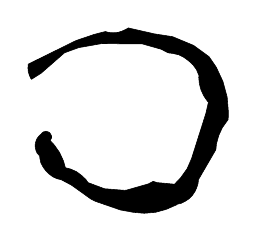
\begin{tikzpicture}[x=1mm,y=1mm,scale=0.041]
                        \begin{scope}[shift={(-190.875,-10.875)}]
  \begin{scope}[draw=black,line join=round,line width=0.208pt]
      \path[draw,fill] (192.0000,473.0000) -- (192.0000,472.0000) --
        (191.0000,461.0000) -- (192.0000,450.0000) -- (195.0000,440.0000) --
        (199.0000,430.0000) -- (202.0000,426.0000) -- (232.0000,445.0000) --
        (303.0000,507.0000) -- (304.0000,508.0000) -- (348.0000,524.0000) --
        (422.0000,537.0000) -- (479.0000,536.0000) -- (482.0000,536.0000) --
        (544.0000,536.0000) -- (604.0000,519.0000) -- (625.0000,508.0000) --
        (640.0000,506.0000) -- (658.0000,502.0000) -- (674.0000,494.0000) --
        (689.0000,483.0000) -- (702.0000,471.0000) -- (713.0000,456.0000) --
        (720.0000,439.0000) -- (721.0000,439.0000) -- (720.0000,432.0000) --
        (722.0000,412.0000) -- (727.0000,393.0000) -- (736.0000,374.0000) --
        (747.0000,358.0000) -- (750.0000,355.0000) -- (742.0000,320.0000) --
        (702.0000,194.0000) -- (698.0000,181.0000) -- (684.0000,149.0000) --
        (664.0000,121.0000) -- (645.0000,101.0000) -- (591.0000,106.0000) --
        (579.0000,110.0000) -- (564.0000,102.0000) -- (501.0000,84.0000) --
        (498.0000,83.0000) -- (490.0000,82.0000) -- (428.0000,87.0000) --
        (377.0000,106.0000) -- (370.0000,116.0000) -- (356.0000,129.0000) --
        (341.0000,140.0000) -- (323.0000,148.0000) -- (307.0000,152.0000) --
        (301.0000,173.0000) -- (289.0000,199.0000) -- (273.0000,222.0000) --
        (260.0000,236.0000) -- (261.0000,239.0000) -- (263.0000,242.0000) --
        (264.0000,244.0000) -- (264.0000,247.0000) -- (264.0000,250.0000) --
        (263.0000,253.0000) -- (261.0000,256.0000) -- (260.0000,258.0000) --
        (258.0000,261.0000) -- (255.0000,262.0000) -- (252.0000,264.0000) --
        (250.0000,264.0000) -- (247.0000,265.0000) -- (244.0000,264.0000) --
        (241.0000,264.0000) -- (238.0000,262.0000) -- (236.0000,261.0000) --
        (233.0000,258.0000) -- (232.0000,256.0000) -- (229.0000,254.0000) --
        (224.0000,249.0000) -- (219.0000,242.0000) -- (216.0000,235.0000) --
        (214.0000,228.0000) -- (213.0000,220.0000) -- (214.0000,213.0000) --
        (216.0000,205.0000) -- (219.0000,198.0000) -- (224.0000,192.0000) --
        (227.0000,189.0000) -- (228.0000,181.0000) -- (231.0000,167.0000) --
        (238.0000,154.0000) -- (246.0000,143.0000) -- (256.0000,133.0000) --
        (268.0000,124.0000) -- (281.0000,118.0000) -- (294.0000,115.0000) --
        (326.0000,98.0000) -- (386.0000,55.0000) -- (400.0000,48.0000) --
        (478.0000,21.0000) -- (507.0000,16.0000) -- (517.0000,14.0000) --
        (551.0000,11.0000) -- (586.0000,14.0000) -- (619.0000,23.0000) --
        (651.0000,37.0000) -- (653.0000,39.0000) -- (666.0000,42.0000) --
        (678.0000,48.0000) -- (690.0000,56.0000) -- (700.0000,66.0000) --
        (708.0000,78.0000) -- (709.0000,80.0000) -- (714.0000,91.0000) --
        (718.0000,104.0000) -- (719.0000,115.0000) -- (773.0000,208.0000) --
        (775.0000,227.0000) -- (782.0000,252.0000) -- (793.0000,276.0000) --
        (808.0000,297.0000) -- (811.0000,301.0000) -- (812.0000,322.0000) --
        (808.0000,371.0000) -- (795.0000,419.0000) -- (774.0000,464.0000) --
        (752.0000,496.0000) -- (704.0000,531.0000) -- (639.0000,558.0000) --
        (581.0000,567.0000) -- (577.0000,568.0000) -- (502.0000,585.0000) --
        (495.0000,581.0000) -- (482.0000,575.0000) -- (469.0000,571.0000) --
        (455.0000,570.0000) -- (441.0000,571.0000) -- (431.0000,574.0000) --
        (396.0000,565.0000) -- (340.0000,546.0000) -- (192.0000,473.0000);
  \end{scope}
\end{scope}
 
                    \end{tikzpicture}
                    \caption{Compound's wall surface}
                    \label{fig:comp-wall}
                \end{subfigure}

                \vspace{0.02\textheight}

                \begin{subfigure}[b]{.33\textwidth}
                    \centering
                    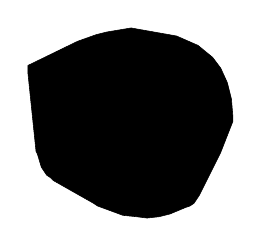
\begin{tikzpicture}[x=1mm,y=1mm,scale=0.17]
                        \begin{scope}[shift={(-419.87,-133.87)}]
  \begin{scope}[draw=black,fill=black,line join=round,line width=0.208pt]
      \path[draw,fill] (497.0000,276.0000) -- (479.0000,273.0000) --
        (471.0000,271.0000) -- (457.0000,266.0000) -- (420.0000,248.0000) --
        (420.0000,245.0000) -- (420.0000,242.0000) -- (426.0000,184.0000) --
        (427.0000,182.0000) -- (430.0000,172.0000) -- (432.0000,169.0000) --
        (434.0000,166.0000) -- (437.0000,164.0000) -- (439.0000,162.0000) --
        (469.0000,145.0000) -- (472.0000,143.0000) -- (491.0000,136.0000) --
        (501.0000,135.0000) -- (509.0000,134.0000) -- (518.0000,135.0000) --
        (526.0000,137.0000) -- (538.0000,142.0000) -- (541.0000,143.0000) --
        (544.0000,145.0000) -- (546.0000,148.0000) -- (548.0000,151.0000) --
        (564.0000,183.0000) -- (573.0000,206.0000) -- (573.0000,211.0000) --
        (572.0000,223.0000) -- (569.0000,235.0000) -- (564.0000,246.0000) --
        (558.0000,254.0000) -- (547.0000,263.0000) -- (531.0000,270.0000) --
        (497.0000,276.0000);
  \end{scope}
\end{scope}
 
                    \end{tikzpicture}
                    \caption{Compound's convex hull}
                    \label{fig:comp-hull}
                \end{subfigure}\hfill\\

                \vspace{0.02\textheight}

                \begin{subfigure}[b]{.33\textwidth}
                    \centering
                    \begin{tikzpicture}[x=1mm,y=1mm,scale=0.045]
                        \begin{scope}[shift={(-191.875,-81.87406)}]
  \begin{scope}[draw=black,fill=c3cad6d,line join=round,line width=0.208pt]
    \path[draw,fill] (192.0000,450.0000) -- (214.0000,213.0000) --
      (213.0000,220.0000) -- (214.0000,228.0000) -- (216.0000,235.0000) --
      (219.0000,242.0000) -- (224.0000,249.0000) -- (229.0000,254.0000) --
      (232.0000,256.0000) -- (233.0000,258.0000) -- (236.0000,261.0000) --
      (238.0000,262.0000) -- (241.0000,264.0000) -- (244.0000,264.0000) --
      (247.0000,265.0000) -- (250.0000,264.0000) -- (252.0000,264.0000) --
      (255.0000,262.0000) -- (258.0000,261.0000) -- (260.0000,258.0000) --
      (261.0000,256.0000) -- (263.0000,253.0000) -- (264.0000,250.0000) --
      (264.0000,247.0000) -- (264.0000,244.0000) -- (263.0000,242.0000) --
      (261.0000,239.0000) -- (260.0000,236.0000) -- (273.0000,222.0000) --
      (289.0000,199.0000) -- (301.0000,173.0000) -- (307.0000,152.0000) --
      (323.0000,148.0000) -- (341.0000,140.0000) -- (356.0000,129.0000) --
      (370.0000,116.0000) -- (377.0000,106.0000) -- (428.0000,87.0000) --
      (490.0000,82.0000) -- (498.0000,83.0000) -- (501.0000,84.0000) --
      (564.0000,102.0000) -- (579.0000,110.0000) -- (591.0000,106.0000) --
      (645.0000,101.0000) -- (664.0000,121.0000) -- (684.0000,149.0000) --
      (698.0000,181.0000) -- (702.0000,194.0000) -- (742.0000,320.0000) --
      (750.0000,355.0000) -- (747.0000,358.0000) -- (736.0000,374.0000) --
      (727.0000,393.0000) -- (722.0000,412.0000) -- (720.0000,432.0000) --
      (721.0000,439.0000) -- (720.0000,439.0000) -- (713.0000,456.0000) --
      (702.0000,471.0000) -- (689.0000,483.0000) -- (674.0000,494.0000) --
      (658.0000,502.0000) -- (640.0000,506.0000) -- (625.0000,508.0000) --
      (604.0000,519.0000) -- (544.0000,536.0000) -- (482.0000,536.0000) --
      (479.0000,536.0000) -- (422.0000,537.0000) -- (348.0000,524.0000) --
      (304.0000,508.0000) -- (303.0000,507.0000) -- (232.0000,445.0000) --
      (202.0000,426.0000) -- (199.0000,430.0000) -- (195.0000,440.0000) --
      (192.0000,450.0000);
  \end{scope}
  \begin{scope}[draw=black,fill=c3cad6d,line join=round,line width=0.208pt]
  \end{scope}
  \begin{scope}[draw=black,fill=c3cad6d,line join=round,line width=0.208pt]
  \end{scope}
  \begin{scope}[draw=black,fill=c3cad6d,line join=round,line width=0.208pt]
  \end{scope}
  \begin{scope}[draw=black,fill=c3cad6d,line join=round,line width=0.208pt]
  \end{scope}
\end{scope}
\begin{scope}[shift={(-191.875,-81.87406)},draw=cff0000,line width=0.800pt]
\end{scope}
 
                    \end{tikzpicture}
                    \caption{Compound's internal surface}
                    \label{fig:comp-area}
                \end{subfigure}\hfill\\

                \vspace{0.02\textheight}

                \begin{subfigure}[b]{.33\textwidth}
                    \centering
                    \begin{tikzpicture}[x=1mm,y=1mm,scale=0.07]
                        \begin{scope}[shift={(-276.875,48.125)}]
  \begin{scope}[draw=black,fill=c88bdb2,line join=round,line width=0.208pt]
      \path[draw,fill] (277.0000,171.0000) -- (305.0000,68.0000) -- (307.0000,68.0000)
        -- (309.0000,67.0000) -- (311.0000,67.0000) -- (312.0000,65.0000) --
        (314.0000,64.0000) -- (315.0000,62.0000) -- (316.0000,61.0000) --
        (316.0000,59.0000) -- (316.0000,57.0000) -- (316.0000,55.0000) --
        (316.0000,53.0000) -- (315.0000,51.0000) -- (314.0000,50.0000) --
        (329.0000,31.0000) -- (341.0000,8.0000) -- (344.0000,-3.0000) --
        (355.0000,-6.0000) -- (366.0000,-11.0000) -- (370.0000,-14.0000) --
        (375.0000,-21.0000) -- (382.0000,-28.0000) -- (390.0000,-33.0000) --
        (398.0000,-37.0000) -- (406.0000,-40.0000) -- (428.0000,-46.0000) --
        (451.0000,-48.0000) -- (467.0000,-47.0000) -- (469.0000,-47.0000) --
        (509.0000,-35.0000) -- (518.0000,-30.0000) -- (526.0000,-32.0000) --
        (561.0000,-36.0000) -- (580.0000,-13.0000) -- (582.0000,-11.0000) --
        (602.0000,34.0000) -- (609.0000,55.0000) -- (623.0000,104.0000) --
        (628.0000,126.0000) -- (626.0000,128.0000) -- (619.0000,138.0000) --
        (614.0000,150.0000) -- (610.0000,163.0000) -- (609.0000,176.0000) --
        (609.0000,180.0000) -- (604.0000,190.0000) -- (597.0000,200.0000) --
        (589.0000,208.0000) -- (580.0000,215.0000) -- (569.0000,220.0000) --
        (558.0000,223.0000) -- (548.0000,224.0000) -- (546.0000,225.0000) --
        (524.0000,235.0000) -- (501.0000,242.0000) -- (476.0000,244.0000) --
        (472.0000,244.0000) -- (438.0000,242.0000) -- (428.0000,243.0000) --
        (418.0000,243.0000) -- (370.0000,234.0000) -- (366.0000,233.0000) --
        (365.0000,233.0000) -- (355.0000,230.0000) -- (345.0000,226.0000) --
        (337.0000,220.0000) -- (330.0000,213.0000) -- (326.0000,208.0000) --
        (296.0000,184.0000) -- (277.0000,171.0000);
  \end{scope}
\end{scope}
\begin{scope}[shift={(-276.875,48.125)},draw=cff0000,line width=0.800pt]
\end{scope}

 
                    \end{tikzpicture}
                    \caption{Correct internal surface}
                    \label{fig:comp-ang-area}
                \end{subfigure}

                \caption[Deriving compound area from difference between total occupied surface and wall surface]{The area derived from the difference between compound's total occupied surface and the wall surface.}
                \label{fig:comp}

                \vspace{-0.07\textheight}
            \end{wrapfigure}

            After distinguishing ditches from compounds, efforts have been focused on geometric data deriving. One of the most useful operations when analyzing settlements is to calculate the area enclosed in ditches or compounds. Unlike some cases published in literature (e.g.\ the area calculation of rectangular shaped \emph{longhouses} \cite{spatial-south-europe}), the present study has to deal with buried, irregularly shaped, rounded compounds.

            The simplest possible approach to compound's area calculation using standard GIS tools can be summarized as follows:
            
            \begin{enumerate}
                \item generate the convex hull\footnote{In mathematics, the convex hull or convex envelope of a set X of points in the Euclidean plane or Euclidean space is the smallest convex set that contains X \cite{wiki:hull}.} of the compound
                \item subtract the surface occupied by the compound wall from the convex hull area
                \item get the extent of the new geometry (in effect, the extension of the compound's internal area)
            \end{enumerate}

            This method has some drawbacks, mostly the needing to fix the limits of the doorway. A sample result using this approach can be seen in \fref{fig:comp} (compound from the Trecasette settlement). The result shows that it is not suitable for analysis, since doorstep is not set adequately (compare \fref{fig:comp-area} with the \ref{fig:comp-ang-area} from % TODO cite angelica
            ). Iterating over this method on all the compounds would have generated a consistent error so this method has been discarded.

            The problem has been solved applying a common analytic geometry procedure, considering the compound's internal surface as the envelope of the compound wall's points nearest to an inner point (the compound's \emph{centroid}). Compound's inner side points have been captured as the intersection between the compound's wall and a new segment binding the centroid with a point external to the compound. Rotating this external points by \SI{1}{\degree}, the segment itself is rotated and the intersection with the innermost point of the compound's wall is registered. This process is explained in \fref{fig:comp-iter}.
            
            In \fref{fig:comp-iter-1} centroid $C$ is calculated using standard GIS tools from compound's convex hull; point $F$ represents the point on the compound's wall with the maximum distance from $C$; point $B$ is obtained applying a buffer to $F$ ($d_{(C,B)} > d_{(C,F)}$). This last step ensures that the circle $D$ created from $B$ --- using $C$ as center --- is outside the compound's geometry (\fref{fig:comp-iter-2}). A set of points is created on $D$ dividing the perimeter by 360, obtaining one point every \SI{1}{\degree}. In detail, given an angle $\alpha$, a circle $D$ with radius $r=d_{(C,B)}$ and center in $C$ ($x_C, y_C$), a general point $P$ ($x_P, y_P$) on $D$ is defined by:
            %
            \begin{align}
                \label{eq:point-circle}
                x_P &= x_C + r\cdot\cos\alpha\\
                y_P &= y_C + r\cdot\sin\alpha
            \end{align}
            %
            In \fref{fig:comp-iter-2} the operation has been repeated with $\alpha=\alpha+1$ for 360 times, obtaining the coordinates of 360 $p_n$ points on circle $D$ (the whole set of points is named $P$). Tracing a line between $C$ and any of the points in $P$ will create a segment (in \fref{fig:comp-iter-3} it is named $CP_1$). If an intersection between this segment and the compound's geometry exists, the innermost point is calculated getting its distance from $C$:
            %
            \begin{align}
                \label{eq:innerpoint}
                d_{i_2 C} < d_{i_1 C}
            \end{align}
            %
            Coordinates of $i_2$ ($x_{i_2}, y_{i_2}$) are saved, since it is the nearest. Iterating this process for all the points $p_n\in P$ will create a new set $I$ of $i_n$ points defining the internal side of the compound's geometry; it could be represented using set theory \cite{molenaar2003} as:
            %
            \begin{align}
                \label{inter-set}
                I = \{ i_1 (x_{i_1}, y_{i_1}), i_2 (x_{i_2}, y_{i_2}), i_3 (x_{i_3}, y_{i_3}), i_n (x_{i_n}, y_{i_n}), \ldots \}
            \end{align}
            %
            In a last step (not represented in \fref{fig:comp-iter}) a convex hull is generated using all the points in $I$; this is the compound's inner surface.

            \begin{figure}
                \centering
                \begin{subfigure}[b]{.5\columnwidth}
                    \centering
                    \begin{tikzpicture}[x=2.5pt,y=2.5pt,scale=0.1
                            %,overlay,shift={(-500,-65)}
                            ]
                        % load base compound path
\begin{scope}[shift={(-190.875,-10.875)}]
  \begin{scope}[draw=black,fill=c0f7296,line join=round,line width=0.208pt]
      \path[draw,fill] (192.0000,473.0000) -- (192.0000,472.0000) --
        (191.0000,461.0000) -- (192.0000,450.0000) -- (195.0000,440.0000) --
        (199.0000,430.0000) -- (202.0000,426.0000) -- (232.0000,445.0000) --
        (303.0000,507.0000) -- (304.0000,508.0000) -- (348.0000,524.0000) --
        (422.0000,537.0000) -- (479.0000,536.0000) -- (482.0000,536.0000) --
        (544.0000,536.0000) -- (604.0000,519.0000) -- (625.0000,508.0000) --
        (640.0000,506.0000) -- (658.0000,502.0000) -- (674.0000,494.0000) --
        (689.0000,483.0000) -- (702.0000,471.0000) -- (713.0000,456.0000) --
        (720.0000,439.0000) -- (721.0000,439.0000) -- (720.0000,432.0000) --
        (722.0000,412.0000) -- (727.0000,393.0000) -- (736.0000,374.0000) --
        (747.0000,358.0000) -- (750.0000,355.0000) -- (742.0000,320.0000) --
        (702.0000,194.0000) -- (698.0000,181.0000) -- (684.0000,149.0000) --
        (664.0000,121.0000) -- (645.0000,101.0000) -- (591.0000,106.0000) --
        (579.0000,110.0000) -- (564.0000,102.0000) -- (501.0000,84.0000) --
        (498.0000,83.0000) -- (490.0000,82.0000) -- (428.0000,87.0000) --
        (377.0000,106.0000) -- (370.0000,116.0000) -- (356.0000,129.0000) --
        (341.0000,140.0000) -- (323.0000,148.0000) -- (307.0000,152.0000) --
        (301.0000,173.0000) -- (289.0000,199.0000) -- (273.0000,222.0000) --
        (260.0000,236.0000) -- (261.0000,239.0000) -- (263.0000,242.0000) --
        (264.0000,244.0000) -- (264.0000,247.0000) -- (264.0000,250.0000) --
        (263.0000,253.0000) -- (261.0000,256.0000) -- (260.0000,258.0000) --
        (258.0000,261.0000) -- (255.0000,262.0000) -- (252.0000,264.0000) --
        (250.0000,264.0000) -- (247.0000,265.0000) -- (244.0000,264.0000) --
        (241.0000,264.0000) -- (238.0000,262.0000) -- (236.0000,261.0000) --
        (233.0000,258.0000) -- (232.0000,256.0000) -- (229.0000,254.0000) --
        (224.0000,249.0000) -- (219.0000,242.0000) -- (216.0000,235.0000) --
        (214.0000,228.0000) -- (213.0000,220.0000) -- (214.0000,213.0000) --
        (216.0000,205.0000) -- (219.0000,198.0000) -- (224.0000,192.0000) --
        (227.0000,189.0000) -- (228.0000,181.0000) -- (231.0000,167.0000) --
        (238.0000,154.0000) -- (246.0000,143.0000) -- (256.0000,133.0000) --
        (268.0000,124.0000) -- (281.0000,118.0000) -- (294.0000,115.0000) --
        (326.0000,98.0000) -- (386.0000,55.0000) -- (400.0000,48.0000) --
        (478.0000,21.0000) -- (507.0000,16.0000) -- (517.0000,14.0000) --
        (551.0000,11.0000) -- (586.0000,14.0000) -- (619.0000,23.0000) --
        (651.0000,37.0000) -- (653.0000,39.0000) -- (666.0000,42.0000) --
        (678.0000,48.0000) -- (690.0000,56.0000) -- (700.0000,66.0000) --
        (708.0000,78.0000) -- (709.0000,80.0000) -- (714.0000,91.0000) --
        (718.0000,104.0000) -- (719.0000,115.0000) -- (773.0000,208.0000) --
        (775.0000,227.0000) -- (782.0000,252.0000) -- (793.0000,276.0000) --
        (808.0000,297.0000) -- (811.0000,301.0000) -- (812.0000,322.0000) --
        (808.0000,371.0000) -- (795.0000,419.0000) -- (774.0000,464.0000) --
        (752.0000,496.0000) -- (704.0000,531.0000) -- (639.0000,558.0000) --
        (581.0000,567.0000) -- (577.0000,568.0000) -- (502.0000,585.0000) --
        (495.0000,581.0000) -- (482.0000,575.0000) -- (469.0000,571.0000) --
        (455.0000,570.0000) -- (441.0000,571.0000) -- (431.0000,574.0000) --
        (396.0000,565.0000) -- (340.0000,546.0000) -- (192.0000,473.0000);
  \end{scope}
\end{scope}
\begin{scope}[shift={(-190.875,-10.875)},draw=cff0000,line width=0.800pt]
\end{scope}


\draw (537.0000,298.0000) circle (0.5cm) coordinate(centr);
\draw (359.0000,210.0000) circle (0.5cm) coordinate(far);
\draw (334.0000,190.0000) circle (0.5cm) coordinate(buf);

\node[left=-0.5pt] at (centr) {\scriptsize C};
\node[above] at (far) {\scriptsize F};
\node[below=0.5pt] at (buf) {\scriptsize B};

\draw (far) -- (buf);
 
                    \end{tikzpicture}
                    \caption{$C$, $F$ and $B$ are calculated.}
                    \label{fig:comp-iter-1}
                \end{subfigure}\\
                \vspace{0.03\textheight}
                \begin{subfigure}[b]{.5\columnwidth}
                    \centering
                    \begin{tikzpicture}[x=2.5pt,y=2.5pt,scale=0.1]
                        % load styles
% styles
\tikzset{snap/.style={circle, draw=blue!50, fill=blue!20, inner sep=0, minimum size=4pt}}
\tikzset{regular/.style={circle, draw=black, fill=white, inner sep=0, minimum size=3pt}}



% load base compound path
\begin{scope}[shift={(-190.875,-10.875)}]
  \begin{scope}[draw=black,fill=c0f7296,line join=round,line width=0.208pt]
      \path[draw,fill] (192.0000,473.0000) -- (192.0000,472.0000) --
        (191.0000,461.0000) -- (192.0000,450.0000) -- (195.0000,440.0000) --
        (199.0000,430.0000) -- (202.0000,426.0000) -- (232.0000,445.0000) --
        (303.0000,507.0000) -- (304.0000,508.0000) -- (348.0000,524.0000) --
        (422.0000,537.0000) -- (479.0000,536.0000) -- (482.0000,536.0000) --
        (544.0000,536.0000) -- (604.0000,519.0000) -- (625.0000,508.0000) --
        (640.0000,506.0000) -- (658.0000,502.0000) -- (674.0000,494.0000) --
        (689.0000,483.0000) -- (702.0000,471.0000) -- (713.0000,456.0000) --
        (720.0000,439.0000) -- (721.0000,439.0000) -- (720.0000,432.0000) --
        (722.0000,412.0000) -- (727.0000,393.0000) -- (736.0000,374.0000) --
        (747.0000,358.0000) -- (750.0000,355.0000) -- (742.0000,320.0000) --
        (702.0000,194.0000) -- (698.0000,181.0000) -- (684.0000,149.0000) --
        (664.0000,121.0000) -- (645.0000,101.0000) -- (591.0000,106.0000) --
        (579.0000,110.0000) -- (564.0000,102.0000) -- (501.0000,84.0000) --
        (498.0000,83.0000) -- (490.0000,82.0000) -- (428.0000,87.0000) --
        (377.0000,106.0000) -- (370.0000,116.0000) -- (356.0000,129.0000) --
        (341.0000,140.0000) -- (323.0000,148.0000) -- (307.0000,152.0000) --
        (301.0000,173.0000) -- (289.0000,199.0000) -- (273.0000,222.0000) --
        (260.0000,236.0000) -- (261.0000,239.0000) -- (263.0000,242.0000) --
        (264.0000,244.0000) -- (264.0000,247.0000) -- (264.0000,250.0000) --
        (263.0000,253.0000) -- (261.0000,256.0000) -- (260.0000,258.0000) --
        (258.0000,261.0000) -- (255.0000,262.0000) -- (252.0000,264.0000) --
        (250.0000,264.0000) -- (247.0000,265.0000) -- (244.0000,264.0000) --
        (241.0000,264.0000) -- (238.0000,262.0000) -- (236.0000,261.0000) --
        (233.0000,258.0000) -- (232.0000,256.0000) -- (229.0000,254.0000) --
        (224.0000,249.0000) -- (219.0000,242.0000) -- (216.0000,235.0000) --
        (214.0000,228.0000) -- (213.0000,220.0000) -- (214.0000,213.0000) --
        (216.0000,205.0000) -- (219.0000,198.0000) -- (224.0000,192.0000) --
        (227.0000,189.0000) -- (228.0000,181.0000) -- (231.0000,167.0000) --
        (238.0000,154.0000) -- (246.0000,143.0000) -- (256.0000,133.0000) --
        (268.0000,124.0000) -- (281.0000,118.0000) -- (294.0000,115.0000) --
        (326.0000,98.0000) -- (386.0000,55.0000) -- (400.0000,48.0000) --
        (478.0000,21.0000) -- (507.0000,16.0000) -- (517.0000,14.0000) --
        (551.0000,11.0000) -- (586.0000,14.0000) -- (619.0000,23.0000) --
        (651.0000,37.0000) -- (653.0000,39.0000) -- (666.0000,42.0000) --
        (678.0000,48.0000) -- (690.0000,56.0000) -- (700.0000,66.0000) --
        (708.0000,78.0000) -- (709.0000,80.0000) -- (714.0000,91.0000) --
        (718.0000,104.0000) -- (719.0000,115.0000) -- (773.0000,208.0000) --
        (775.0000,227.0000) -- (782.0000,252.0000) -- (793.0000,276.0000) --
        (808.0000,297.0000) -- (811.0000,301.0000) -- (812.0000,322.0000) --
        (808.0000,371.0000) -- (795.0000,419.0000) -- (774.0000,464.0000) --
        (752.0000,496.0000) -- (704.0000,531.0000) -- (639.0000,558.0000) --
        (581.0000,567.0000) -- (577.0000,568.0000) -- (502.0000,585.0000) --
        (495.0000,581.0000) -- (482.0000,575.0000) -- (469.0000,571.0000) --
        (455.0000,570.0000) -- (441.0000,571.0000) -- (431.0000,574.0000) --
        (396.0000,565.0000) -- (340.0000,546.0000) -- (192.0000,473.0000);
  \end{scope}
\end{scope}
\begin{scope}[shift={(-190.875,-10.875)},draw=cff0000,line width=0.800pt]
\end{scope}


% nodes
\node[regular]   (buf)   at  (334.0000,190.0000)    {};
\node[regular]   (centr) at  (537.0000,298.0000)    {};

% set the polar coordinates center to the (centr) point
\begin{scope}[shift=(centr)]

    \foreach \name/\idx/\angle in {snap3/4/0, snap2/3/30, snap1/2/60, snap0/1/90}
    \draw   let
                \p1 = (buf),
                \p2 = (centr),
                \n1 = {veclen((\x2-\x1),(\y2+\y1))}
            in
                node[snap] (\name) at (\angle:\n1)          {}
                node[color=blue] at (\angle:\n1 + 80pt) {\scriptsize $P_\idx$};
\end{scope}

% circle
\node[draw,dashed,circle through=(buf),label=left:{\scriptsize D}] at (centr) {};

% labels
\node[left=0.5pt] at (centr) {\scriptsize C};
\node[below=0.5pt] at (buf) {\scriptsize B};
 
                    \end{tikzpicture}
                    \caption{Points $P_n$ on $D$, created from $B$.}
                    \label{fig:comp-iter-2}
                \end{subfigure}\\
                \vspace{0.03\textheight}
                \begin{subfigure}[b]{.5\columnwidth}
                    \centering
                    \begin{tikzpicture}[x=2.5pt,y=2.5pt,scale=0.1]
                        % define styles
\tikzset{i-1/.style={circle,
                       draw=blue,
                       fill=blue,
                       inner sep=0,
                       minimum size=3pt,
                       pin=280:\tiny $i_\s$,
                       },
         i-2/.style={circle,
                       draw=red,
                       fill=red,
                       inner sep=0,
                       minimum size=3pt,
                       pin=80:\tiny $i_\s$,
                       }
}

\begin{scope}
    [spy using overlays={circle,
                         blue,
                         magnification=2,
                         size=50pt,
                         connect spies}]

    % load previous graph
    % load styles
% styles
\tikzset{snap/.style={circle, draw=blue!50, fill=blue!20, inner sep=0, minimum size=4pt}}
\tikzset{regular/.style={circle, draw=black, fill=white, inner sep=0, minimum size=3pt}}



% load base compound path
\begin{scope}[shift={(-190.875,-10.875)}]
  \begin{scope}[draw=black,fill=c0f7296,line join=round,line width=0.208pt]
      \path[draw,fill] (192.0000,473.0000) -- (192.0000,472.0000) --
        (191.0000,461.0000) -- (192.0000,450.0000) -- (195.0000,440.0000) --
        (199.0000,430.0000) -- (202.0000,426.0000) -- (232.0000,445.0000) --
        (303.0000,507.0000) -- (304.0000,508.0000) -- (348.0000,524.0000) --
        (422.0000,537.0000) -- (479.0000,536.0000) -- (482.0000,536.0000) --
        (544.0000,536.0000) -- (604.0000,519.0000) -- (625.0000,508.0000) --
        (640.0000,506.0000) -- (658.0000,502.0000) -- (674.0000,494.0000) --
        (689.0000,483.0000) -- (702.0000,471.0000) -- (713.0000,456.0000) --
        (720.0000,439.0000) -- (721.0000,439.0000) -- (720.0000,432.0000) --
        (722.0000,412.0000) -- (727.0000,393.0000) -- (736.0000,374.0000) --
        (747.0000,358.0000) -- (750.0000,355.0000) -- (742.0000,320.0000) --
        (702.0000,194.0000) -- (698.0000,181.0000) -- (684.0000,149.0000) --
        (664.0000,121.0000) -- (645.0000,101.0000) -- (591.0000,106.0000) --
        (579.0000,110.0000) -- (564.0000,102.0000) -- (501.0000,84.0000) --
        (498.0000,83.0000) -- (490.0000,82.0000) -- (428.0000,87.0000) --
        (377.0000,106.0000) -- (370.0000,116.0000) -- (356.0000,129.0000) --
        (341.0000,140.0000) -- (323.0000,148.0000) -- (307.0000,152.0000) --
        (301.0000,173.0000) -- (289.0000,199.0000) -- (273.0000,222.0000) --
        (260.0000,236.0000) -- (261.0000,239.0000) -- (263.0000,242.0000) --
        (264.0000,244.0000) -- (264.0000,247.0000) -- (264.0000,250.0000) --
        (263.0000,253.0000) -- (261.0000,256.0000) -- (260.0000,258.0000) --
        (258.0000,261.0000) -- (255.0000,262.0000) -- (252.0000,264.0000) --
        (250.0000,264.0000) -- (247.0000,265.0000) -- (244.0000,264.0000) --
        (241.0000,264.0000) -- (238.0000,262.0000) -- (236.0000,261.0000) --
        (233.0000,258.0000) -- (232.0000,256.0000) -- (229.0000,254.0000) --
        (224.0000,249.0000) -- (219.0000,242.0000) -- (216.0000,235.0000) --
        (214.0000,228.0000) -- (213.0000,220.0000) -- (214.0000,213.0000) --
        (216.0000,205.0000) -- (219.0000,198.0000) -- (224.0000,192.0000) --
        (227.0000,189.0000) -- (228.0000,181.0000) -- (231.0000,167.0000) --
        (238.0000,154.0000) -- (246.0000,143.0000) -- (256.0000,133.0000) --
        (268.0000,124.0000) -- (281.0000,118.0000) -- (294.0000,115.0000) --
        (326.0000,98.0000) -- (386.0000,55.0000) -- (400.0000,48.0000) --
        (478.0000,21.0000) -- (507.0000,16.0000) -- (517.0000,14.0000) --
        (551.0000,11.0000) -- (586.0000,14.0000) -- (619.0000,23.0000) --
        (651.0000,37.0000) -- (653.0000,39.0000) -- (666.0000,42.0000) --
        (678.0000,48.0000) -- (690.0000,56.0000) -- (700.0000,66.0000) --
        (708.0000,78.0000) -- (709.0000,80.0000) -- (714.0000,91.0000) --
        (718.0000,104.0000) -- (719.0000,115.0000) -- (773.0000,208.0000) --
        (775.0000,227.0000) -- (782.0000,252.0000) -- (793.0000,276.0000) --
        (808.0000,297.0000) -- (811.0000,301.0000) -- (812.0000,322.0000) --
        (808.0000,371.0000) -- (795.0000,419.0000) -- (774.0000,464.0000) --
        (752.0000,496.0000) -- (704.0000,531.0000) -- (639.0000,558.0000) --
        (581.0000,567.0000) -- (577.0000,568.0000) -- (502.0000,585.0000) --
        (495.0000,581.0000) -- (482.0000,575.0000) -- (469.0000,571.0000) --
        (455.0000,570.0000) -- (441.0000,571.0000) -- (431.0000,574.0000) --
        (396.0000,565.0000) -- (340.0000,546.0000) -- (192.0000,473.0000);
  \end{scope}
\end{scope}
\begin{scope}[shift={(-190.875,-10.875)},draw=cff0000,line width=0.800pt]
\end{scope}


% nodes
\node[regular]   (buf)   at  (334.0000,190.0000)    {};
\node[regular]   (centr) at  (537.0000,298.0000)    {};

% set the polar coordinates center to the (centr) point
\begin{scope}[shift=(centr)]

    \foreach \name/\idx/\angle in {snap3/4/0, snap2/3/30, snap1/2/60, snap0/1/90}
    \draw   let
                \p1 = (buf),
                \p2 = (centr),
                \n1 = {veclen((\x2-\x1),(\y2+\y1))}
            in
                node[snap] (\name) at (\angle:\n1)          {}
                node[color=blue] at (\angle:\n1 + 80pt) {\scriptsize $P_\idx$};
\end{scope}

% circle
\node[draw,dashed,circle through=(buf),label=left:{\scriptsize D}] at (centr) {};

% labels
\node[left=0.5pt] at (centr) {\scriptsize C};
\node[below=0.5pt] at (buf) {\scriptsize B};


    \begin{scope}[shift=(centr)]
        % add segment from center to point on external circle
        \draw [name path=centr-snap3] (centr) -- (snap3);

        % draw nodes on intersections
        \fill [name intersections={of=centr-snap3 and compound, name=i}]
        \foreach \s in {1,2}{
            (i-\s) node[i-\s] {}
        };

        % add spy magnification
        \spy on ($ (i-1)!.5!(i-2) $) in node (zoom) [right] at (600,-40);
    \end{scope}
\end{scope}
 
                    \end{tikzpicture}
                    \caption{Each $P$: save inner intersection ($i_2$).}
                    \label{fig:comp-iter-3}
                \end{subfigure}\\
                \vspace{0.03\textheight}
                \begin{subfigure}[b]{.5\columnwidth}
                    \centering
                    \begin{tikzpicture}[x=2.5pt,y=2.5pt,scale=0.1
                            %,overlay,shift={(-500,130)}
                            ]
                        \begin{scope}[
              every path/.style={
                decoration={
                    markings,
                    mark=between positions 0.57 and 1.2 step 6pt with {
                        \fill[red] circle (2pt);
                    }
                }
              }
]
    % load base compound path
    \begin{scope}[shift={(-190.875,-10.875)}]
  \begin{scope}[draw=black,fill=c0f7296,line join=round,line width=0.208pt]
      \path[draw,fill] (192.0000,473.0000) -- (192.0000,472.0000) --
        (191.0000,461.0000) -- (192.0000,450.0000) -- (195.0000,440.0000) --
        (199.0000,430.0000) -- (202.0000,426.0000) -- (232.0000,445.0000) --
        (303.0000,507.0000) -- (304.0000,508.0000) -- (348.0000,524.0000) --
        (422.0000,537.0000) -- (479.0000,536.0000) -- (482.0000,536.0000) --
        (544.0000,536.0000) -- (604.0000,519.0000) -- (625.0000,508.0000) --
        (640.0000,506.0000) -- (658.0000,502.0000) -- (674.0000,494.0000) --
        (689.0000,483.0000) -- (702.0000,471.0000) -- (713.0000,456.0000) --
        (720.0000,439.0000) -- (721.0000,439.0000) -- (720.0000,432.0000) --
        (722.0000,412.0000) -- (727.0000,393.0000) -- (736.0000,374.0000) --
        (747.0000,358.0000) -- (750.0000,355.0000) -- (742.0000,320.0000) --
        (702.0000,194.0000) -- (698.0000,181.0000) -- (684.0000,149.0000) --
        (664.0000,121.0000) -- (645.0000,101.0000) -- (591.0000,106.0000) --
        (579.0000,110.0000) -- (564.0000,102.0000) -- (501.0000,84.0000) --
        (498.0000,83.0000) -- (490.0000,82.0000) -- (428.0000,87.0000) --
        (377.0000,106.0000) -- (370.0000,116.0000) -- (356.0000,129.0000) --
        (341.0000,140.0000) -- (323.0000,148.0000) -- (307.0000,152.0000) --
        (301.0000,173.0000) -- (289.0000,199.0000) -- (273.0000,222.0000) --
        (260.0000,236.0000) -- (261.0000,239.0000) -- (263.0000,242.0000) --
        (264.0000,244.0000) -- (264.0000,247.0000) -- (264.0000,250.0000) --
        (263.0000,253.0000) -- (261.0000,256.0000) -- (260.0000,258.0000) --
        (258.0000,261.0000) -- (255.0000,262.0000) -- (252.0000,264.0000) --
        (250.0000,264.0000) -- (247.0000,265.0000) -- (244.0000,264.0000) --
        (241.0000,264.0000) -- (238.0000,262.0000) -- (236.0000,261.0000) --
        (233.0000,258.0000) -- (232.0000,256.0000) -- (229.0000,254.0000) --
        (224.0000,249.0000) -- (219.0000,242.0000) -- (216.0000,235.0000) --
        (214.0000,228.0000) -- (213.0000,220.0000) -- (214.0000,213.0000) --
        (216.0000,205.0000) -- (219.0000,198.0000) -- (224.0000,192.0000) --
        (227.0000,189.0000) -- (228.0000,181.0000) -- (231.0000,167.0000) --
        (238.0000,154.0000) -- (246.0000,143.0000) -- (256.0000,133.0000) --
        (268.0000,124.0000) -- (281.0000,118.0000) -- (294.0000,115.0000) --
        (326.0000,98.0000) -- (386.0000,55.0000) -- (400.0000,48.0000) --
        (478.0000,21.0000) -- (507.0000,16.0000) -- (517.0000,14.0000) --
        (551.0000,11.0000) -- (586.0000,14.0000) -- (619.0000,23.0000) --
        (651.0000,37.0000) -- (653.0000,39.0000) -- (666.0000,42.0000) --
        (678.0000,48.0000) -- (690.0000,56.0000) -- (700.0000,66.0000) --
        (708.0000,78.0000) -- (709.0000,80.0000) -- (714.0000,91.0000) --
        (718.0000,104.0000) -- (719.0000,115.0000) -- (773.0000,208.0000) --
        (775.0000,227.0000) -- (782.0000,252.0000) -- (793.0000,276.0000) --
        (808.0000,297.0000) -- (811.0000,301.0000) -- (812.0000,322.0000) --
        (808.0000,371.0000) -- (795.0000,419.0000) -- (774.0000,464.0000) --
        (752.0000,496.0000) -- (704.0000,531.0000) -- (639.0000,558.0000) --
        (581.0000,567.0000) -- (577.0000,568.0000) -- (502.0000,585.0000) --
        (495.0000,581.0000) -- (482.0000,575.0000) -- (469.0000,571.0000) --
        (455.0000,570.0000) -- (441.0000,571.0000) -- (431.0000,574.0000) --
        (396.0000,565.0000) -- (340.0000,546.0000) -- (192.0000,473.0000);
  \end{scope}
\end{scope}
\begin{scope}[shift={(-190.875,-10.875)},draw=cff0000,line width=0.800pt]
\end{scope}

\end{scope}
 
                    \end{tikzpicture}
                    \caption{$i_n\in I$ inner intersection points.}
                    \label{fig:comp-iter-4}
                \end{subfigure}

                %\begin{subfigure}[b]{.5\columnwidth}
                %    \centering
                %    \begin{tikzpicture}[x=2.5pt,y=2.5pt,scale=0.09
                %            %,overlay,shift={(-500,130)}
                %            ]
                %        \input{img/comp-iter-5} 
                %    \end{tikzpicture}
                %    \caption{$i_n\in I$ inner intersection points.}
                %    \label{fig:comp-iter-5}
                %\end{subfigure}

                \caption[Derivation of compound's internal surface using analytic geometry]{Derivation of compound's internal surface in 4 steps, using analytic geometry.}
                \label{fig:comp-iter}
            \end{figure}
            
            A Python algorithm has been used to automate the process, which saves the derived area geometries to a database table separated from the others. Further informations could be derived from these geometries, mostly their perimeter and surface in \si{\meter\squared} (they are saved as attributes). A sample table with the compound's area and attributes is presented in \fref{tab:tab-area-anglisano}. The derived perimeters and areas are useful for a comparison with the results obtained from a manual deriving of the same data % TODO cite angelica
            .

            \begin{table}
                \centering
                \begin{tabular}{ccccc}
    \toprule
    ID & shapefile\_id & perimeter & area & type\\
    \otoprule
    1 & 1 & 54.231591 & 204.520791 & compound\\
    4 & 1 & 100.294549 & 551.619397 & compound\\
    6 & 1 & 49.230435 & 171.483569 & compound\\
    16 & 1 & 816.404075 & 45265.204341 & ditch\\
    \bottomrule
\end{tabular}

                \caption[Sample results of area geometries derived from compounds and their attributes for the Anglisano settlement.]{Sample results of the derived area geometries for some compounds in the Anglisano settlement. Rows 1, 4 and 16 represent the same compounds as in \fref{tab:jnb-results}, excepted that the perimeter value is calculated from the area geometry and not from the compound's wall geometry as before (the data are not redundant).}
                \label{tab:tab-area-anglisano}
            \end{table}

        \subsection{Automating discovering of compounds access and orientation}

            The current method used to describe compounds' orientation consists of a visual check of the compound's access position relatively to a set of 8 cardinal points (N, NE, E, SE, S, SW, W, NW) % TODO cite angelica
            . The operator had to visually recognize the orientation of the access and write the relative number (from 1 to 8) as an attribute in a Shapefile's field created on purpose; this lead to manually writing a number for each one of the compounds for all the sites. It is a time-consuming activity that could be automated.

            Literature reports few cases in which orientation has been calculated automatically using GIS methods. In most cases, the analyzed settlements present \emph{houses} more than \emph{compounds}: these have a nearly regular --- mostly rectangular --- shape, in which the orientation can be easily taken as the angle between cardinal north and house's longest axis \cite[p.~53]{spatial-south-europe}. Unfortunately, this is not the case, since compounds have a really irregular shape and in most cases the geometry's longer axis is not meaningful.

            The orientation of an object with respect of a cardinal point can be defined as the angle between the cardinal north and a representative feature of the object (e.g.\ the main axis). When analyzing compounds, this feature is the access.
            \subsubsection{Finding the compound's access}
                \begin{wrapfigure}{r}{0.45\textwidth}
                    \vspace{-0.08\textheight}
                    \centering
                    \begin{tikzpicture}[x=1mm,y=1mm,scale=0.005]
                        \input{tab/dot-flow-access}
                    \end{tikzpicture}
                    \caption[Logic process to determine the compound's access.]{Finding compound's access vertexes. The flow exits when the last point of the $I$ set is reached: $d$ contains the longest side.}
                    \label{fig:flow-access}
                    \vspace{-0.04\textheight}
                \end{wrapfigure}

                The proposed approach depends entirely from the derived areas geometries (\fref{sec:comp-area}): the observation led to consider as an access the longest straight side of the geometry. In other words, the farthest couple of points will identify compound's access (as it is easy to observe in \fref{fig:comp-iter-4}).
                
                The solution consists of an iteration on all the points in the above mentioned $I$ set of points, comparing each couple of points' distance with the one of the previous couple; the longest distance is registered. This process is better explained in \fref{fig:flow-access}: after getting the first point in the $I$ intersections set, a default distance of $d=0$ is defined; if the distance between the current point and the next is more than $d$, this value is assigned to $d$ itself. Then, the current point is shifted to the next and the next one is taken, and the process is repeated. When the last point in the $I$ set is reached, $d$ will contain the maximum registered distance (the compound's access), and $i_n$ one vertex of the access (the other is simply $i_{n+1}$). The resulting access vertexes for the compound in \fref{fig:comp-iter} are represented as $a_1, a_2$ in \fref{fig:comp-orient-1}.

            \subsubsection{Finding the access orientation}
                %
                %\begin{figure}
                \begin{wrapfigure}{r}{0.45\textwidth}
                    \vspace{-0.08\textheight}
                    \centering
                    \begin{subfigure}[b]{.4\columnwidth}
                        \centering
                        \begin{tikzpicture}[x=2.5pt,y=2.5pt,scale=0.09]
                            % load styles
% styles
\tikzset{snap/.style={circle, draw=blue!50, fill=blue!20, inner sep=0, minimum size=4pt}}
\tikzset{regular/.style={circle, draw=black, fill=white, inner sep=0, minimum size=3pt}}



% load base compound path
\begin{scope}[shift={(-190.875,-10.875)}]
  \begin{scope}[draw=black,fill=c0f7296,line join=round,line width=0.208pt]
      \path[draw,fill] (192.0000,473.0000) -- (192.0000,472.0000) --
        (191.0000,461.0000) -- (192.0000,450.0000) -- (195.0000,440.0000) --
        (199.0000,430.0000) -- (202.0000,426.0000) -- (232.0000,445.0000) --
        (303.0000,507.0000) -- (304.0000,508.0000) -- (348.0000,524.0000) --
        (422.0000,537.0000) -- (479.0000,536.0000) -- (482.0000,536.0000) --
        (544.0000,536.0000) -- (604.0000,519.0000) -- (625.0000,508.0000) --
        (640.0000,506.0000) -- (658.0000,502.0000) -- (674.0000,494.0000) --
        (689.0000,483.0000) -- (702.0000,471.0000) -- (713.0000,456.0000) --
        (720.0000,439.0000) -- (721.0000,439.0000) -- (720.0000,432.0000) --
        (722.0000,412.0000) -- (727.0000,393.0000) -- (736.0000,374.0000) --
        (747.0000,358.0000) -- (750.0000,355.0000) -- (742.0000,320.0000) --
        (702.0000,194.0000) -- (698.0000,181.0000) -- (684.0000,149.0000) --
        (664.0000,121.0000) -- (645.0000,101.0000) -- (591.0000,106.0000) --
        (579.0000,110.0000) -- (564.0000,102.0000) -- (501.0000,84.0000) --
        (498.0000,83.0000) -- (490.0000,82.0000) -- (428.0000,87.0000) --
        (377.0000,106.0000) -- (370.0000,116.0000) -- (356.0000,129.0000) --
        (341.0000,140.0000) -- (323.0000,148.0000) -- (307.0000,152.0000) --
        (301.0000,173.0000) -- (289.0000,199.0000) -- (273.0000,222.0000) --
        (260.0000,236.0000) -- (261.0000,239.0000) -- (263.0000,242.0000) --
        (264.0000,244.0000) -- (264.0000,247.0000) -- (264.0000,250.0000) --
        (263.0000,253.0000) -- (261.0000,256.0000) -- (260.0000,258.0000) --
        (258.0000,261.0000) -- (255.0000,262.0000) -- (252.0000,264.0000) --
        (250.0000,264.0000) -- (247.0000,265.0000) -- (244.0000,264.0000) --
        (241.0000,264.0000) -- (238.0000,262.0000) -- (236.0000,261.0000) --
        (233.0000,258.0000) -- (232.0000,256.0000) -- (229.0000,254.0000) --
        (224.0000,249.0000) -- (219.0000,242.0000) -- (216.0000,235.0000) --
        (214.0000,228.0000) -- (213.0000,220.0000) -- (214.0000,213.0000) --
        (216.0000,205.0000) -- (219.0000,198.0000) -- (224.0000,192.0000) --
        (227.0000,189.0000) -- (228.0000,181.0000) -- (231.0000,167.0000) --
        (238.0000,154.0000) -- (246.0000,143.0000) -- (256.0000,133.0000) --
        (268.0000,124.0000) -- (281.0000,118.0000) -- (294.0000,115.0000) --
        (326.0000,98.0000) -- (386.0000,55.0000) -- (400.0000,48.0000) --
        (478.0000,21.0000) -- (507.0000,16.0000) -- (517.0000,14.0000) --
        (551.0000,11.0000) -- (586.0000,14.0000) -- (619.0000,23.0000) --
        (651.0000,37.0000) -- (653.0000,39.0000) -- (666.0000,42.0000) --
        (678.0000,48.0000) -- (690.0000,56.0000) -- (700.0000,66.0000) --
        (708.0000,78.0000) -- (709.0000,80.0000) -- (714.0000,91.0000) --
        (718.0000,104.0000) -- (719.0000,115.0000) -- (773.0000,208.0000) --
        (775.0000,227.0000) -- (782.0000,252.0000) -- (793.0000,276.0000) --
        (808.0000,297.0000) -- (811.0000,301.0000) -- (812.0000,322.0000) --
        (808.0000,371.0000) -- (795.0000,419.0000) -- (774.0000,464.0000) --
        (752.0000,496.0000) -- (704.0000,531.0000) -- (639.0000,558.0000) --
        (581.0000,567.0000) -- (577.0000,568.0000) -- (502.0000,585.0000) --
        (495.0000,581.0000) -- (482.0000,575.0000) -- (469.0000,571.0000) --
        (455.0000,570.0000) -- (441.0000,571.0000) -- (431.0000,574.0000) --
        (396.0000,565.0000) -- (340.0000,546.0000) -- (192.0000,473.0000);
  \end{scope}
\end{scope}
\begin{scope}[shift={(-190.875,-10.875)},draw=cff0000,line width=0.800pt]
\end{scope}


% points of interest
\draw (537.0000,298.0000) circle (0.5cm) coordinate(centr);
\node[below right=0.2pt] at (centr) {\scriptsize C};

\node[regular]   (buf)   at  (334.0000,190.0000)    {};
\node[below=0.5pt] at (buf) {\scriptsize B};

% access points
\draw[draw=red,fill=red] (379.0000,230.0000) circle (20pt) coordinate(acc-n);
\draw[draw=red,fill=red] (389.0000,360.0000) circle (20pt) coordinate(acc-s);

\node[right=-0.5pt] at (acc-s) {\scriptsize $a_1$};
\node[right=-0.5pt] at (acc-n) {\scriptsize $a_2$};

% access line with centroid
\draw (acc-n) -- (acc-s);

\node[circle,inner sep=0pt,minimum size=3pt,fill=blue
    %,pin=150:\tiny centroid
    ] (centroid) at ($ (acc-n)!.5!(acc-s) $) {};
\node[right] (centroid-label) at (centroid) {\scriptsize $e$};
 
                        \end{tikzpicture}
                        \caption{Centroid $e$ is derived from access segment.}
                        \label{fig:comp-orient-1}
                    \end{subfigure}\\
                    \vspace{0.02\textheight}
                    \begin{subfigure}[b]{.4\columnwidth}
                        \centering
                        \begin{tikzpicture}[x=2.5pt,y=2.5pt,scale=0.09]
                            % load styles
% styles
\tikzset{snap/.style={circle, draw=blue!50, fill=blue!20, inner sep=0, minimum size=4pt}}
\tikzset{regular/.style={circle, draw=black, fill=white, inner sep=0, minimum size=3pt}}



% load base compound path
\begin{scope}[shift={(-190.875,-10.875)}]
  \begin{scope}[draw=black,fill=c0f7296,line join=round,line width=0.208pt]
      \path[draw,fill] (192.0000,473.0000) -- (192.0000,472.0000) --
        (191.0000,461.0000) -- (192.0000,450.0000) -- (195.0000,440.0000) --
        (199.0000,430.0000) -- (202.0000,426.0000) -- (232.0000,445.0000) --
        (303.0000,507.0000) -- (304.0000,508.0000) -- (348.0000,524.0000) --
        (422.0000,537.0000) -- (479.0000,536.0000) -- (482.0000,536.0000) --
        (544.0000,536.0000) -- (604.0000,519.0000) -- (625.0000,508.0000) --
        (640.0000,506.0000) -- (658.0000,502.0000) -- (674.0000,494.0000) --
        (689.0000,483.0000) -- (702.0000,471.0000) -- (713.0000,456.0000) --
        (720.0000,439.0000) -- (721.0000,439.0000) -- (720.0000,432.0000) --
        (722.0000,412.0000) -- (727.0000,393.0000) -- (736.0000,374.0000) --
        (747.0000,358.0000) -- (750.0000,355.0000) -- (742.0000,320.0000) --
        (702.0000,194.0000) -- (698.0000,181.0000) -- (684.0000,149.0000) --
        (664.0000,121.0000) -- (645.0000,101.0000) -- (591.0000,106.0000) --
        (579.0000,110.0000) -- (564.0000,102.0000) -- (501.0000,84.0000) --
        (498.0000,83.0000) -- (490.0000,82.0000) -- (428.0000,87.0000) --
        (377.0000,106.0000) -- (370.0000,116.0000) -- (356.0000,129.0000) --
        (341.0000,140.0000) -- (323.0000,148.0000) -- (307.0000,152.0000) --
        (301.0000,173.0000) -- (289.0000,199.0000) -- (273.0000,222.0000) --
        (260.0000,236.0000) -- (261.0000,239.0000) -- (263.0000,242.0000) --
        (264.0000,244.0000) -- (264.0000,247.0000) -- (264.0000,250.0000) --
        (263.0000,253.0000) -- (261.0000,256.0000) -- (260.0000,258.0000) --
        (258.0000,261.0000) -- (255.0000,262.0000) -- (252.0000,264.0000) --
        (250.0000,264.0000) -- (247.0000,265.0000) -- (244.0000,264.0000) --
        (241.0000,264.0000) -- (238.0000,262.0000) -- (236.0000,261.0000) --
        (233.0000,258.0000) -- (232.0000,256.0000) -- (229.0000,254.0000) --
        (224.0000,249.0000) -- (219.0000,242.0000) -- (216.0000,235.0000) --
        (214.0000,228.0000) -- (213.0000,220.0000) -- (214.0000,213.0000) --
        (216.0000,205.0000) -- (219.0000,198.0000) -- (224.0000,192.0000) --
        (227.0000,189.0000) -- (228.0000,181.0000) -- (231.0000,167.0000) --
        (238.0000,154.0000) -- (246.0000,143.0000) -- (256.0000,133.0000) --
        (268.0000,124.0000) -- (281.0000,118.0000) -- (294.0000,115.0000) --
        (326.0000,98.0000) -- (386.0000,55.0000) -- (400.0000,48.0000) --
        (478.0000,21.0000) -- (507.0000,16.0000) -- (517.0000,14.0000) --
        (551.0000,11.0000) -- (586.0000,14.0000) -- (619.0000,23.0000) --
        (651.0000,37.0000) -- (653.0000,39.0000) -- (666.0000,42.0000) --
        (678.0000,48.0000) -- (690.0000,56.0000) -- (700.0000,66.0000) --
        (708.0000,78.0000) -- (709.0000,80.0000) -- (714.0000,91.0000) --
        (718.0000,104.0000) -- (719.0000,115.0000) -- (773.0000,208.0000) --
        (775.0000,227.0000) -- (782.0000,252.0000) -- (793.0000,276.0000) --
        (808.0000,297.0000) -- (811.0000,301.0000) -- (812.0000,322.0000) --
        (808.0000,371.0000) -- (795.0000,419.0000) -- (774.0000,464.0000) --
        (752.0000,496.0000) -- (704.0000,531.0000) -- (639.0000,558.0000) --
        (581.0000,567.0000) -- (577.0000,568.0000) -- (502.0000,585.0000) --
        (495.0000,581.0000) -- (482.0000,575.0000) -- (469.0000,571.0000) --
        (455.0000,570.0000) -- (441.0000,571.0000) -- (431.0000,574.0000) --
        (396.0000,565.0000) -- (340.0000,546.0000) -- (192.0000,473.0000);
  \end{scope}
\end{scope}
\begin{scope}[shift={(-190.875,-10.875)},draw=cff0000,line width=0.800pt]
\end{scope}


% points of interest
\draw (537.0000,298.0000) circle (0.5cm) coordinate(centr);

% access points
\draw[] (379.0000,230.0000) circle (20pt) coordinate(acc-n);
\draw[] (389.0000,360.0000) circle (20pt) coordinate(acc-s);

% access line with centroid
\draw (acc-n) -- (acc-s);
\node[circle,inner sep=0pt,minimum size=3pt,fill=blue] (centroid) at ($ (acc-n)!.5!(acc-s) $) {};

% set the polar coordinates center to the (centr) point
\begin{scope}[shift=(centr)]

    \foreach \name/\angle in {a/45+22.5, b/90+22.5, c/135+22.5, d/180+22.5, e/225+22.5, f/270+22.5, g/315+22.5, h/360+22.5}
    \draw   let
                \p1 = (buf),
                \p2 = (centr),
                \n1 = {veclen((\x2-\x1),(\y2+\y1))}
            in
                node[snap] (\name) at (\angle:\n1)          {}
                node[color=blue] (ang-\name) at (\angle:\n1 + 80pt) {};
\end{scope}

% path to draw octagon
\path[dashed,draw=blue!40]  (a)   edge    node[above,blue]      {\tiny N}   (b)
                            (b)   edge    node[above left,blue] {\tiny NW}  (c)
                            (c)   edge    node[left,blue]       {\tiny W}   (d)
                            (d)   edge    node[below left,blue] {\tiny SW}  (e)
                            (e)   edge    node[below,blue]      {\tiny S}   (f)
                            (f)   edge    node[below right,blue]{\tiny SE}  (g)
                            (g)   edge    node[right,blue]      {\tiny E}   (h)
                            (h)   edge    node[above right,blue]{\tiny NE}  (a);

% draw octagon's slice
\path[draw=blue!30] (centr) -- (e);
\path[draw=blue!30] (centr) -- (f);

\node[below=10pt,blue] (angle) at (centr) {\tiny $\alpha$};

% sample point coordinates
\node[above right,blue] (sample-coord) at (a) {\tiny $x_p$, $y_p$};

                        \end{tikzpicture}
                        \caption{Cardinal points with $\alpha=\sfrac{360}{8}=\SI{45}{\degree}$, built from $B$.}
                        \label{fig:comp-orient-2}
                    \end{subfigure}
                    \vspace{0.02\textheight}
                    \begin{subfigure}[b]{.4\columnwidth}
                        \centering
                        \begin{tikzpicture}[x=2.5pt,y=2.5pt,scale=0.09]
                            % load styles
% styles
\tikzset{snap/.style={circle, draw=blue!50, fill=blue!20, inner sep=0, minimum size=4pt}}
\tikzset{regular/.style={circle, draw=black, fill=white, inner sep=0, minimum size=3pt}}



% load base compound path
\begin{scope}[shift={(-190.875,-10.875)}]
  \begin{scope}[draw=black,fill=c0f7296,line join=round,line width=0.208pt]
      \path[draw,fill] (192.0000,473.0000) -- (192.0000,472.0000) --
        (191.0000,461.0000) -- (192.0000,450.0000) -- (195.0000,440.0000) --
        (199.0000,430.0000) -- (202.0000,426.0000) -- (232.0000,445.0000) --
        (303.0000,507.0000) -- (304.0000,508.0000) -- (348.0000,524.0000) --
        (422.0000,537.0000) -- (479.0000,536.0000) -- (482.0000,536.0000) --
        (544.0000,536.0000) -- (604.0000,519.0000) -- (625.0000,508.0000) --
        (640.0000,506.0000) -- (658.0000,502.0000) -- (674.0000,494.0000) --
        (689.0000,483.0000) -- (702.0000,471.0000) -- (713.0000,456.0000) --
        (720.0000,439.0000) -- (721.0000,439.0000) -- (720.0000,432.0000) --
        (722.0000,412.0000) -- (727.0000,393.0000) -- (736.0000,374.0000) --
        (747.0000,358.0000) -- (750.0000,355.0000) -- (742.0000,320.0000) --
        (702.0000,194.0000) -- (698.0000,181.0000) -- (684.0000,149.0000) --
        (664.0000,121.0000) -- (645.0000,101.0000) -- (591.0000,106.0000) --
        (579.0000,110.0000) -- (564.0000,102.0000) -- (501.0000,84.0000) --
        (498.0000,83.0000) -- (490.0000,82.0000) -- (428.0000,87.0000) --
        (377.0000,106.0000) -- (370.0000,116.0000) -- (356.0000,129.0000) --
        (341.0000,140.0000) -- (323.0000,148.0000) -- (307.0000,152.0000) --
        (301.0000,173.0000) -- (289.0000,199.0000) -- (273.0000,222.0000) --
        (260.0000,236.0000) -- (261.0000,239.0000) -- (263.0000,242.0000) --
        (264.0000,244.0000) -- (264.0000,247.0000) -- (264.0000,250.0000) --
        (263.0000,253.0000) -- (261.0000,256.0000) -- (260.0000,258.0000) --
        (258.0000,261.0000) -- (255.0000,262.0000) -- (252.0000,264.0000) --
        (250.0000,264.0000) -- (247.0000,265.0000) -- (244.0000,264.0000) --
        (241.0000,264.0000) -- (238.0000,262.0000) -- (236.0000,261.0000) --
        (233.0000,258.0000) -- (232.0000,256.0000) -- (229.0000,254.0000) --
        (224.0000,249.0000) -- (219.0000,242.0000) -- (216.0000,235.0000) --
        (214.0000,228.0000) -- (213.0000,220.0000) -- (214.0000,213.0000) --
        (216.0000,205.0000) -- (219.0000,198.0000) -- (224.0000,192.0000) --
        (227.0000,189.0000) -- (228.0000,181.0000) -- (231.0000,167.0000) --
        (238.0000,154.0000) -- (246.0000,143.0000) -- (256.0000,133.0000) --
        (268.0000,124.0000) -- (281.0000,118.0000) -- (294.0000,115.0000) --
        (326.0000,98.0000) -- (386.0000,55.0000) -- (400.0000,48.0000) --
        (478.0000,21.0000) -- (507.0000,16.0000) -- (517.0000,14.0000) --
        (551.0000,11.0000) -- (586.0000,14.0000) -- (619.0000,23.0000) --
        (651.0000,37.0000) -- (653.0000,39.0000) -- (666.0000,42.0000) --
        (678.0000,48.0000) -- (690.0000,56.0000) -- (700.0000,66.0000) --
        (708.0000,78.0000) -- (709.0000,80.0000) -- (714.0000,91.0000) --
        (718.0000,104.0000) -- (719.0000,115.0000) -- (773.0000,208.0000) --
        (775.0000,227.0000) -- (782.0000,252.0000) -- (793.0000,276.0000) --
        (808.0000,297.0000) -- (811.0000,301.0000) -- (812.0000,322.0000) --
        (808.0000,371.0000) -- (795.0000,419.0000) -- (774.0000,464.0000) --
        (752.0000,496.0000) -- (704.0000,531.0000) -- (639.0000,558.0000) --
        (581.0000,567.0000) -- (577.0000,568.0000) -- (502.0000,585.0000) --
        (495.0000,581.0000) -- (482.0000,575.0000) -- (469.0000,571.0000) --
        (455.0000,570.0000) -- (441.0000,571.0000) -- (431.0000,574.0000) --
        (396.0000,565.0000) -- (340.0000,546.0000) -- (192.0000,473.0000);
  \end{scope}
\end{scope}
\begin{scope}[shift={(-190.875,-10.875)},draw=cff0000,line width=0.800pt]
\end{scope}


% points of interest
\draw (537.0000,298.0000) circle (0.5cm) coordinate(centr);

% access points
\draw[] (379.0000,230.0000) circle (20pt) coordinate(acc-n);
\draw[] (389.0000,360.0000) circle (20pt) coordinate(acc-s);

% access line with centroid
\draw (acc-n) -- (acc-s);
\node[circle,inner sep=0pt,minimum size=3pt,fill=blue] (centroid) at ($ (acc-n)!.5!(acc-s) $) {};

% set the polar coordinates center to the (centr) point
\begin{scope}[shift=(centr)]

    \foreach \name/\angle in {a/45+22.5, b/90+22.5, c/135+22.5, d/180+22.5, e/225+22.5, f/270+22.5, g/315+22.5, h/360+22.5}
    \draw   let
                \p1 = (buf),
                \p2 = (centr),
                \n1 = {veclen((\x2-\x1),(\y2+\y1))}
            in
                node[] (\name) at (\angle:\n1)          {}
                node[color=blue] (ang-\name) at (\angle:\n1 + 80pt) {};
\end{scope}

\path[dashed,draw=blue!40]  (a)   edge    node[above,blue]      {}   (b)
                            (b)   edge    node[above left,blue] {}  (c)
                            (c)   edge    node[left=6pt,blue,fill=YellowGreen!40,rounded corners]       {\tiny W}   (d)
                            (d)   edge    node[below left,blue] {}  (e)
                            (e)   edge    node[below,blue]      {}   (f)
                            (f)   edge    node[below right,blue]{}  (g)
                            (g)   edge    node[right,blue]      {}   (h)
                            (h)   edge    node[above right,blue]{}  (a);

\begin{pgfonlayer}{background}
    \fill[YellowGreen!40] (c) -- (centr) -- (d) -- (c) -- cycle;
    \fill[red!30] (a) -- (centr) -- (b) -- (a) -- cycle;
    \fill[red!30] (b) -- (centr) -- (c) -- (b) -- cycle;
    \fill[red!30] (d) -- (centr) -- (e) -- (d) -- cycle;
    \fill[red!30] (e) -- (centr) -- (f) -- (e) -- cycle;
    \fill[red!30] (f) -- (centr) -- (g) -- (f) -- cycle;
    \fill[red!30] (g) -- (centr) -- (h) -- (g) -- cycle;
    \fill[red!30] (h) -- (centr) -- (a) -- (h) -- cycle;
\end{pgfonlayer}

                        \end{tikzpicture}
                        \caption{$e$ is contained in $W$ area.}
                        \label{fig:comp-orient-3}
                    \end{subfigure}
                    \vspace{0.02\textheight}
                    \begin{subfigure}[b]{.4\columnwidth}
                        \centering
                        \begin{tikzpicture}[x=2.5pt,y=2.5pt,scale=0.09]
                            % load styles
% styles
\tikzset{snap/.style={circle, draw=blue!50, fill=blue!20, inner sep=0, minimum size=4pt}}
\tikzset{regular/.style={circle, draw=black, fill=white, inner sep=0, minimum size=3pt}}



% load base compound path
\begin{scope}[shift={(-190.875,-10.875)}]
  \begin{scope}[draw=black,fill=c0f7296,line join=round,line width=0.208pt]
      \path[draw,fill] (192.0000,473.0000) -- (192.0000,472.0000) --
        (191.0000,461.0000) -- (192.0000,450.0000) -- (195.0000,440.0000) --
        (199.0000,430.0000) -- (202.0000,426.0000) -- (232.0000,445.0000) --
        (303.0000,507.0000) -- (304.0000,508.0000) -- (348.0000,524.0000) --
        (422.0000,537.0000) -- (479.0000,536.0000) -- (482.0000,536.0000) --
        (544.0000,536.0000) -- (604.0000,519.0000) -- (625.0000,508.0000) --
        (640.0000,506.0000) -- (658.0000,502.0000) -- (674.0000,494.0000) --
        (689.0000,483.0000) -- (702.0000,471.0000) -- (713.0000,456.0000) --
        (720.0000,439.0000) -- (721.0000,439.0000) -- (720.0000,432.0000) --
        (722.0000,412.0000) -- (727.0000,393.0000) -- (736.0000,374.0000) --
        (747.0000,358.0000) -- (750.0000,355.0000) -- (742.0000,320.0000) --
        (702.0000,194.0000) -- (698.0000,181.0000) -- (684.0000,149.0000) --
        (664.0000,121.0000) -- (645.0000,101.0000) -- (591.0000,106.0000) --
        (579.0000,110.0000) -- (564.0000,102.0000) -- (501.0000,84.0000) --
        (498.0000,83.0000) -- (490.0000,82.0000) -- (428.0000,87.0000) --
        (377.0000,106.0000) -- (370.0000,116.0000) -- (356.0000,129.0000) --
        (341.0000,140.0000) -- (323.0000,148.0000) -- (307.0000,152.0000) --
        (301.0000,173.0000) -- (289.0000,199.0000) -- (273.0000,222.0000) --
        (260.0000,236.0000) -- (261.0000,239.0000) -- (263.0000,242.0000) --
        (264.0000,244.0000) -- (264.0000,247.0000) -- (264.0000,250.0000) --
        (263.0000,253.0000) -- (261.0000,256.0000) -- (260.0000,258.0000) --
        (258.0000,261.0000) -- (255.0000,262.0000) -- (252.0000,264.0000) --
        (250.0000,264.0000) -- (247.0000,265.0000) -- (244.0000,264.0000) --
        (241.0000,264.0000) -- (238.0000,262.0000) -- (236.0000,261.0000) --
        (233.0000,258.0000) -- (232.0000,256.0000) -- (229.0000,254.0000) --
        (224.0000,249.0000) -- (219.0000,242.0000) -- (216.0000,235.0000) --
        (214.0000,228.0000) -- (213.0000,220.0000) -- (214.0000,213.0000) --
        (216.0000,205.0000) -- (219.0000,198.0000) -- (224.0000,192.0000) --
        (227.0000,189.0000) -- (228.0000,181.0000) -- (231.0000,167.0000) --
        (238.0000,154.0000) -- (246.0000,143.0000) -- (256.0000,133.0000) --
        (268.0000,124.0000) -- (281.0000,118.0000) -- (294.0000,115.0000) --
        (326.0000,98.0000) -- (386.0000,55.0000) -- (400.0000,48.0000) --
        (478.0000,21.0000) -- (507.0000,16.0000) -- (517.0000,14.0000) --
        (551.0000,11.0000) -- (586.0000,14.0000) -- (619.0000,23.0000) --
        (651.0000,37.0000) -- (653.0000,39.0000) -- (666.0000,42.0000) --
        (678.0000,48.0000) -- (690.0000,56.0000) -- (700.0000,66.0000) --
        (708.0000,78.0000) -- (709.0000,80.0000) -- (714.0000,91.0000) --
        (718.0000,104.0000) -- (719.0000,115.0000) -- (773.0000,208.0000) --
        (775.0000,227.0000) -- (782.0000,252.0000) -- (793.0000,276.0000) --
        (808.0000,297.0000) -- (811.0000,301.0000) -- (812.0000,322.0000) --
        (808.0000,371.0000) -- (795.0000,419.0000) -- (774.0000,464.0000) --
        (752.0000,496.0000) -- (704.0000,531.0000) -- (639.0000,558.0000) --
        (581.0000,567.0000) -- (577.0000,568.0000) -- (502.0000,585.0000) --
        (495.0000,581.0000) -- (482.0000,575.0000) -- (469.0000,571.0000) --
        (455.0000,570.0000) -- (441.0000,571.0000) -- (431.0000,574.0000) --
        (396.0000,565.0000) -- (340.0000,546.0000) -- (192.0000,473.0000);
  \end{scope}
\end{scope}
\begin{scope}[shift={(-190.875,-10.875)},draw=cff0000,line width=0.800pt]
\end{scope}


% points of interest
\draw (537.0000,298.0000) circle (0.5cm) coordinate(centr);

% access points
\draw[] (379.0000,230.0000) circle (20pt) coordinate(acc-n);
\draw[] (389.0000,360.0000) circle (20pt) coordinate(acc-s);

% access line with centroid
\draw (acc-n) -- (acc-s);
\node[circle,inner sep=0pt,minimum size=3pt,fill=blue] (centroid) at ($ (acc-n)!.5!(acc-s) $) {};

% set the polar coordinates center to the (centr) point
\begin{scope}[shift=(centr)]

    \foreach \name/\angle in {a/45+22.5, b/90+22.5, c/135+22.5, d/180+22.5, e/225+22.5, f/270+22.5, g/315+22.5, h/360+22.5}
    \draw   let
                \p1 = (buf),
                \p2 = (centr),
                \n1 = {veclen((\x2-\x1),(\y2+\y1))}
            in
                node[] (\name) at (\angle:\n1)          {}
                node[color=blue] (ang-\name) at (\angle:\n1 + 80pt) {};
\end{scope}

\path[dashed,draw=blue!40]  (a)   edge    node[above,blue]      {}   (b)
                            (b)   edge    node[above left,blue] {}  (c)
                            (c)   edge    node[left=6pt,blue,fill=YellowGreen!40,rounded corners]       {\tiny W}   (d)
                            (d)   edge    node[below left,blue] {}  (e)
                            (e)   edge    node[below,blue]      {}   (f)
                            (f)   edge    node[below right,blue]{}  (g)
                            (g)   edge    node[right,blue]      {}   (h)
                            (h)   edge    node[above right,blue]{}  (a);

\begin{pgfonlayer}{background}
    \fill[YellowGreen!40] (c) -- (centr) -- (d) -- (c) -- cycle;
    \fill[red!30] (a) -- (centr) -- (b) -- (a) -- cycle;
    \fill[red!30] (b) -- (centr) -- (c) -- (b) -- cycle;
    \fill[red!30] (d) -- (centr) -- (e) -- (d) -- cycle;
    \fill[red!30] (e) -- (centr) -- (f) -- (e) -- cycle;
    \fill[red!30] (f) -- (centr) -- (g) -- (f) -- cycle;
    \fill[red!30] (g) -- (centr) -- (h) -- (g) -- cycle;
    \fill[red!30] (h) -- (centr) -- (a) -- (h) -- cycle;
\end{pgfonlayer}


\path[dashed,draw=blue!40]  (a)   edge    node[above,blue]      {\scriptsize 2}   (b)
                            (b)   edge    node[above left,blue] {\scriptsize 3}  (c)
                            (c)   edge    node[left=6pt,blue,fill=YellowGreen!40,rounded corners]       {\scriptsize 4}   (d)
                            (d)   edge    node[below left,blue] {\scriptsize 5}  (e)
                            (e)   edge    node[below,blue]      {\scriptsize 6}   (f)
                            (f)   edge    node[below right,blue]{\scriptsize 7}  (g)
                            (g)   edge    node[right,blue]      {\scriptsize 0}   (h)
                            (h)   edge    node[above right,blue]{\scriptsize 1}  (a);

\begin{pgfonlayer}{background}
    \fill[YellowGreen!40] (c) -- (centr) -- (d) -- (c) -- cycle;
    \fill[white] (a) -- (centr) -- (b) -- (a) -- cycle;
    \fill[white] (b) -- (centr) -- (c) -- (b) -- cycle;
    \fill[white] (d) -- (centr) -- (e) -- (d) -- cycle;
    \fill[white] (e) -- (centr) -- (f) -- (e) -- cycle;
    \fill[white] (f) -- (centr) -- (g) -- (f) -- cycle;
    \fill[white] (g) -- (centr) -- (h) -- (g) -- cycle;
    \fill[white] (h) -- (centr) -- (a) -- (h) -- cycle;
\end{pgfonlayer}

                        \end{tikzpicture}
                        \caption{A numerical index is assigned to every cardinal point (in this case, $W=4$).}
                        \label{fig:comp-orient-4}
                    \end{subfigure}

                    \caption[Graphical rapresentation of the steps to derive compound's access orientation.]{Derivation of the orientation for a single compound's access segment.% While $a_1, a_2 \in I$, $e$ is derived using GIS.
                    }
                    \label{fig:comp-orient}
                    \vspace{-0.1\textheight}
                \end{wrapfigure}
                %
                Since the access (or doorstep) of a compound is the segment joining the two farthest points in its internal surface ($a_1$, $a_2$), we can derive compound's orientation as the orientation of this segment. Many approaches are possible; we have chosen to calculate the cardinal point that ``contains'' the access. The calculation consisted in building an octagon using the 8 above mentioned cardinal points as sides. Every triangular slice of the octagon represents the area for that cardinal point. Then, a simple \emph{spatial} check of which triangle contains the access segment allows to define the orientation of the access. This process details are represented in \fref{fig:comp-orient}.
                
                Unfortunately, some compounds have a very large access, so we need to reduce the access to a smaller geometry: we considered the access segment's centroid. This point is calculated using standard GIS tools; from the geometrical point of view, the centroid of a line is its \emph{midpoint} \cite{calculus-geom}; for a line segment joining $P_1$ $(x_1, y_1)$ and $P_2$ $(x_2, y_2)$ the midpoint $(\bar{x}, \bar{y})$ is
                %
                \begin{align}
                    \label{eq:midpoint}
                    \left(\bar{x}, \bar{y}\right) = \left(\frac{1}{2}\left(x_1 + x_2\right),\frac{1}{2}\left(y_1 + y_2\right)\right)
                \end{align}
                %
                Considering $P_1 = a_1$ and $P_2 = a_2$, $e$ is obtained (\fref{fig:comp-orient-1}).
                
                The calculation of the bounding octagon has been operated using the buffered point $B$ (see \fref{fig:comp-iter-1}) to draw points in \fref{fig:comp-orient-2}. A generic cardinal point $p$ is calculated as in \fref{eq:point-circle}:
                %
                \begin{align}
                    \label{eq:point-cardinal}
                    x_P &= x_C + d_{C,B}\cdot\cos{(\SI{360}{\degree}/8)}\\
                    y_P &= y_C + d_{C,B}\cdot\sin{(\SI{360}{\degree}/8)}
                \end{align}
                
                The last step, in \fref{fig:comp-orient-3} uses a standard \emph{contains} GIS function to determine in which triangle the centroid $e$ is contained, iterating over all triangles; the example returns a western orientation. To ease the statistical approach, a numerical index has been attributed to each cardinal point (e.g.\ $W = 4$ in \fref{fig:comp-orient-4}).

                To store the results, a new table is created; for each compounds the table registers the original Shapefile's ID, the compound's ID, the length of the access segment (automatically calculated as $d_{a_1, a_2}$, and the orientation index (between $0$ and $7$). Sample results for the Anglisano settlements are shown in \fref{tab:tab-access-anglisano}.
                %
                \begin{table}
                    \centering
                    \begin{tabular}{ccccc}
    \toprule
    ID & shapefile ID & comp ID & length & orientation\\
    \otoprule
    1   &   1   &   2   &   11.112974   &   2\\
    6   &   1   &   7   &   6.818017    &   3\\
    10  &   1   &   11  &   22.592364   &   5\\
    16  &   1   &   19  &   32.479378   &   5\\
    \bottomrule
\end{tabular}

                    \caption[Sample results of access calculations for the compounds in the Anglisano settlement.]{Sample results of access calculations for the compounds in the Anglisano settlement.}
                    \label{tab:tab-access-anglisano}
                \end{table}

        \subsection{Development of the open source webGIS interface}

            \begin{figure}[htp]
                \centering
                \resizebox{0.9\textwidth}{!}{%
                    \begin{tikzpicture}[remember picture]
                        \input{tab/dot-geo-workflow-def}
                    \end{tikzpicture}
                }
                \caption[The three diffrent tables to store compound's derived data.]{The new data structure of the Tavoliere project. Starting from the same raster data as in \fref{fig:scheme-derive}, all the newly derived vector data and their attributes are placed in a different table.}
                \label{fig:scheme-derive-2}
            \end{figure}

        %\subsection{Inner/outer compounds}
